% ---------------------------------------------------------------------
% --- Arquivo principal e os demais serao os dos capitulos.
% --- EXPRESSÔES ENTRE <> DEVERÂO SER COMPLETADAS COM A INFORMAÇÂO ESPECÌFICA DO TRABALHO 
% ---------------------------------------------------------------------

% Atualizado para atender as normas ABNT por Mônica da Silva (04/11/2021)

%configuração da entrada 
    % 12pt, 	% tamanho da fonte
    %openright, % capítulos começam em pág ímpar (insere página vazia caso preciso)
    % oneside, %% IMPRESSÃO dos elementos textuais e pós-textuais: oneside (apenas no anverso) ou twoside (anverso e verso, se mais de 100 p.) (insere páginas em branco).
    % a4paper, % tamanho do papel. 
    % english, % idioma adicional para hifenização
   	%english,			% idioma adicional para hifenização
	%french,				% idioma adicional para hifenização
	%spanish,			% idioma adicional para hifenização
	%brazil,				% o último idioma é o principal do documento

\documentclass[ruledheader, 12pt, openright, a4paper, oneside, english, brazil]{PPGC_UFF}
%---pacotes para hiphenizacao e acentuacao em portugues
\usepackage[brazil]{babel}
\usepackage[T1]{fontenc}
\usepackage[utf8]{inputenc}	
%\usepackage[latin1]{inputenc}
\usepackage[utf8]{inputenc}
\usepackage[T1]{fontenc}


%--- pacote para figuras
\usepackage{epsf, subfigure}
\usepackage[dvips]{epsfig,graphicx}
\usepackage{chngcntr} %configuração dos padrões numéricos das Figuras e Tabelas
\counterwithout{figure}{chapter} %formata figura para padrão: Figura 1.
\counterwithout{table}{chapter} %formata tabela para padrão: Tabela 1.


%--- pacote de simbolos
\usepackage{pifont,textcomp,latexsym}

%--- simbolos matematicos
\usepackage{amssymb,amstext,amsthm,icomma,amsmath}

\usepackage [round]{natbib}
\bibliographystyle{dinar}

%--- pacote para gerar pseudo-codigo
\usepackage{algorithm}
\usepackage{algorithmic}
\floatname{algorithm}{Algoritmo}

%--- outros pacotes
\usepackage{url}
\usepackage{longtable}
\usepackage{lscape}
\usepackage{quoting}

%Tabela Colorida
\usepackage{bigdelim,booktabs, colortbl, longtable, multirow, multicol,rotating }



%%===============================================================================
%% INICIO do Pacotes - Lista de abreviaturas, siglas e acrônimos
%%===============================================================================
		
% Modo "file": utiliza os termos definidos no arquivo acronimos.tex
%  1) Inserção tabular da listas
%  2) Controle da ordem de apresentação das listas
%  3) Não é preciso referenciar no texto
% nonumberlist, %do not show page numbers
% acronym,      %generate acronym listing   -> Not used in this example (see line with)
% toc,          % Inclui a abreviatura no sumário e conta pagina
% section]      %use section level for toc entries
\usepackage[acronym,nopostdot,shortcuts, nonumberlist]{glossaries}


\makeglossaries
\newacronym{ONU}{ONU}{Organização das Nações Unidas}
\newacronym{ACR}{ACR}{Acronimos}
\newacronym{CNN}{CNN}{Acronimos}

%%===============================================================================
%% FIM do Pacotes Lista de abreviaturas, siglas e acrônimos
%%===============================================================================

%%===============================================================================
%% Configuração das citações e personalização 
%%===============================================================================

% Os pacotes abaixo só podem ser usados juntamente com o pacote ABNT abaixo e na ordem atual. 
% Esse conjunto de pacotes permite que as citações fiquem na cor azul e sejam usadas como link para as referencias. 
\usepackage[bookmarksopen=true,
            linktoc=page, 
            colorlinks=true,  %ativa a cor do link na referencia
            linkcolor=blue, %muda a cor do link na referencia \ref{} números de tabelas, figuras, seções, sumário etc. 
            citecolor=blue, % muda a cor das citações \cite \textcite
            filecolor=magenta, 
            urlcolor=blue, %muda a cor da url \url no texto e ref. bibliográfica
            ]{hyperref}


\usepackage[ %mais informações de personalização das referencias olhar nos arquivos PDF na pasta MANUAIS OU https://www.overleaf.com/learn/latex/Biblatex_bibliography_styles
    style = abnt, % Sistema alfabético
    %style = abnt-numeric, % Sistema numérico
    %style = abnt-ibid, % Notas de referência
    language=brazil,
    backend=biber,
]{biblatex}

\addbibresource{bibliografia.bib} % A biblioteca para ser utilizada na dissertação/tese.

%%===============================================================================
%% FIM da configuração das citações e personalização 
%%===============================================================================

\hyphenation{
a-de-qua-da-men-te 
di-men-sio-na-men-to 
}

%---------usando tipo de fonte padrão  
% mathptmx (títulos sem negrito) ou ptm (títulos negrito)  - Times - Padrão 
% ugq (títulos negrito) - Arial 
%% --  Padrão do template é: ptm  -- %%
\renewcommand{\ABNTchapterfont}{\bfseries\fontfamily{ptm}\fontseries{b}\selectfont} 
\renewcommand{\ABNTsectionfont}{\bfseries\fontfamily{ptm}}


% --- -----------------------------------------------------------------
% --- Documento Principal.
% --- -----------------------------------------------------------------

\begin{document}


% --- -----------------------------------------------------------------
% --- Titulo, abstract, dedicatórias e agradecimentos.
% --- Índice geral, lista de figuras e tabelas.
% --- -----------------------------------------------------------------
% Atualizado para atender as normas ABNT por Mônica da Silva (04/11/2021)

% --- -----------------------------------------------------------------
% --- Elementos usados na Capa e na Folha de Rosto.
% --- EXPRESSÔES ENTRE <> DEVERÂO SER COMPLETADAS COM A INFORMAÇÂO ESPECÍFICA DO TRABALHO
% --- E OS SÌMBOLOS <> DEVEM SER RETIRADOS 
% --- -----------------------------------------------------------------
\autor{Thiago Augusto Fernandes de Carvalho} % deve ser escrito em maiúsculo

\titulo{Avaliação da fração de ejeção cardíaca em ecocardiogramas utilizando uma rede neural
UViT / Roberta}

\instituicao{UNIVERSIDADE FEDERAL FLUMINENSE}

\orientador{Flávio Luiz Seixas}


\local{NITER\'{O}I}

\data{2024} % ano da defesa

\comentario{Dissertação de Mestrado apresentada ao Programa de P\'{o}s-Gradua\c{c}\~{a}o em Computa\c{c}\~{a}o da \mbox{Universidade} Federal Fluminense como requisito parcial para a obten\c{c}\~{a}o do Grau de \mbox{Mestre em Computa\c{c}\~{a}o}. \'{A}rea de concentra\c{c}\~{a}o: \mbox{Ciência da Computação}} %preencha com a sua área de concentração

% --- -----------------------------------------------------------------
% --- Capa. (Capa externa, aquela com as letrinhas douradas)(Obrigatório)
% --- ----------------------------------------------------------------
\capa

% --- -----------------------------------------------------------------
% --- Folha de rosto. (Obrigatório)
% --- ----------------------------------------------------------------
\folhaderosto

% --- -----------------------------------------------------------------
% --- Ficha catalográfica obrigatória na versão final. (Obrigatório)
% --- ----------------------------------------------------------------



\begin{figure}[!ht]
    \centering
    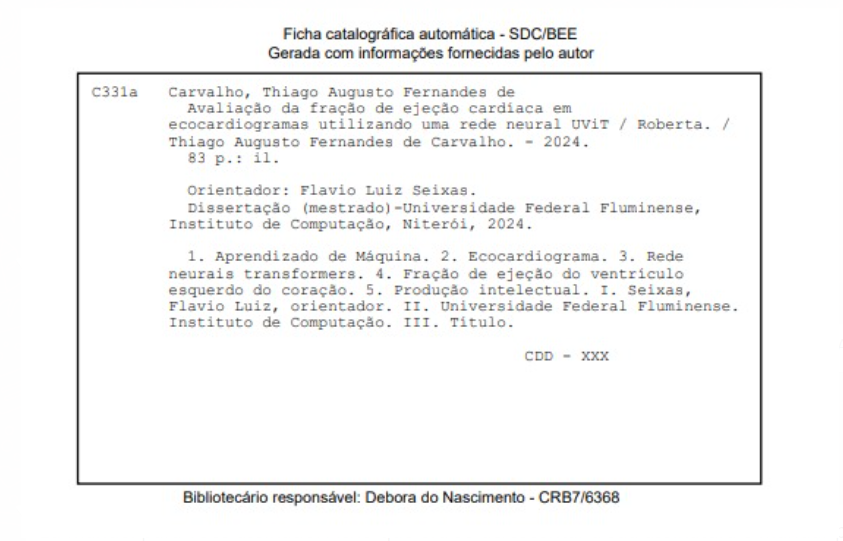
\includegraphics[width=1\linewidth]{capitulos//figuras/fichacarto.png}
    \caption{Ficha catalográfica}
    \label{fig:enter-label}
\end{figure}

\cleardoublepage


\pagestyle{ruledheader}
\setcounter{page}{1}
\pagenumbering{roman}

% --- -----------------------------------------------------------------
% --- Termo de aprovação. (Obrigatório)
% --- ----------------------------------------------------------------
\cleardoublepage
\thispagestyle{empty}

\vspace{-60mm}

\begin{center}
   {\large Thiago Augusto Fernandes de Carvalho}\\
   \vspace{7mm}

  Avaliação da fração de ejeção cardíaca em ecocardiogramas utilizando
uma rede neural UViT / Roberta.\\
  \vspace{10mm}
\end{center}

\noindent
\begin{flushright}
\begin{minipage}[t]{8cm}

Dissertação de Mestrado> apresentada ao Programa de P\'{o}s-Gradua\c{c}\~{a}o em Computa\c{c}\~{a}o da Universidade Federal Fluminense como requisito parcial para a obten\c{c}\~{a}o do \mbox{Grau} de  Mestre em Computa\c{c}\~{a}o. \'{A}rea de concentra\c{c}\~{a}o: \mbox{Ciência da Computação.} %preencha com a sua área de concentração

\end{minipage}
\end{flushright}
\vspace{1.0 cm}
\noindent
Aprovada em  Junho de 2024. \\

\begin{figure}[!ht]
    \centering
    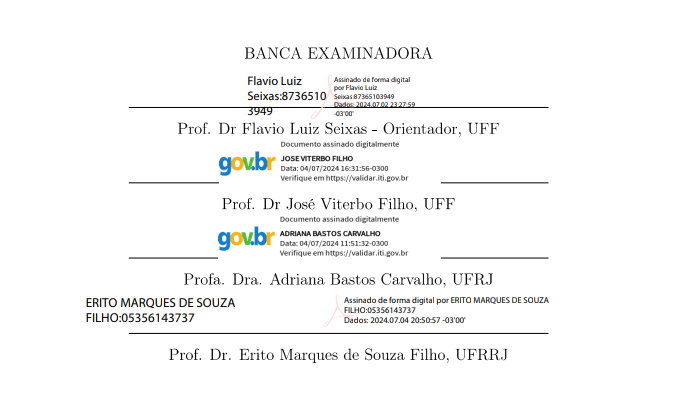
\includegraphics[width=1\linewidth]{capitulos//figuras/assinaturas.png}
    
    \label{fig:enter-label}
\end{figure}
\begin{center}
  \vspace{4mm}
  Niter\'{o}i \\
  %\vspace{6mm}
  2024

\end{center}



% --- -----------------------------------------------------------------
% --- Agradecimentos.(Opcional)
% --- -----------------------------------------------------------------
\pretextualchapter{Agradecimentos}
\hspace{5mm}


Agradeço primeiramente a Deus, pela força e pelas oportunidades únicas que me foram concedidas em minha jornada, e pelos momentos inestimáveis que tenho vivido. Expresso minha profunda gratidão ao meu orientador, pelo conhecimento transmitido, pelo suporte incansável, pelos conselhos sábios e pela paciência durante o desenvolvimento deste trabalho. Aos meus pais, pelo incentivo constante, pela crença inabalável em meu potencial e pelo amor e suporte que são a base de tudo que busco e conquisto. Vocês são minha inspiração e dedico a vocês cada passo que avanço. À minha esposa, companheira leal e fonte de amor e motivação diária. Sua presença é um suporte constante em minha vida, incentivando-me a alcançar meus sonhos e permanecer firme em meus objetivos. Seu apoio é inestimável, e esta conquista também pertence a você. À minha família, avós e tios, pelo afeto profundo e pelo suporte incondicional. Cada um de vocês tem um papel especial em minha vida, contribuindo para a minha felicidade e sucesso. Aos meus amigos e colegas, por serem uma rede de apoio, pelas risadas e momentos compartilhados. Cada um de vocês tem enriquecido minha vida de uma forma única. E a todos os professores e amigos que cruzaram meu caminho, em especial aos que se tornaram mentores e verdadeiros amigos, cujo apoio e incentivo foram cruciais para que eu alcançasse voos mais altos. Esta conquista também é de vocês.


% --- -----------------------------------------------------------------
% --- Resumo em português.(Obrigatório)
% --- -----------------------------------------------------------------
\begin{resumo}


Esta dissertação abordou a necessidade de diagnósticos cardíacos mais confiáveis, cruciais para tratamentos eficazes de diversas condições cardíacas, e focou na otimização de métodos de análise de ecocardiogramas para melhorar a precisão na estimativa da fração de ejeção do ventrículo esquerdo, essencial para diagnósticos cardíacos. Após uma revisão sistemática da literatura e a seleção de conjuntos de dados de ecocardiogramas adultos e pediátricos, a metodologia utilizou uma versão modificada da Ultrassom Video Transformer (UViT), integrando tecnologias como RoBERTa para análise espaço-temporal. A avaliação dos modelos, através de métricas como MAE, RMSE e R², revelou melhorias significativas em relação à bibliografia levantada, especialmente com o modelo RoBERTa, que se destacou em termos de precisão e capacidade de generalização para dados adultos e pediátricos. A pesquisa sugere que a abordagem proposta pode melhorar a precisão diagnóstica e ser aplicada clinicamente, contribuindo para decisões médicas mais informadas. As contribuições incluem um método robusto para análise de ecocardiogramas e abrem caminho para futuros trabalhos em categorização automática de pacientes por idade, melhoria da qualidade de imagens com redes neurais generativas e interpretação automática de relatórios médicos com modelos avançados de linguagem.

{\hspace{-8mm} \bf{Palavras-chave}}: ecocardiograma, fração de ejeção do ventrículo esquerdo, aprendizado profundo, análise de imagens médicas, RoBERTa, DistilBERT.

\end{resumo}

% --- -----------------------------------------------------------------
% --- Resumo em língua estrangeira.(Obrigatório)
% --- -----------------------------------------------------------------
\begin{abstract}

This dissertation addressed the need for more reliable cardiac diagnoses, crucial for effective treatments of various heart conditions, and focused on optimizing echocardiogram analysis methods to improve the accuracy of left ventricular ejection fraction estimation, which is essential for cardiac diagnoses. After a systematic literature review and the selection of adult and pediatric echocardiogram datasets, the methodology utilized a modified version of the Ultrasound Video Transformer (UViT), integrating technologies such as RoBERTa for spatiotemporal analysis. The evaluation of the models, using metrics like MAE, RMSE, and R², revealed significant improvements compared to the reviewed literature, especially with the RoBERTa model, which excelled in terms of accuracy and generalization capacity for both adult and pediatric data. The research suggests that the proposed approach can enhance diagnostic accuracy and be clinically applied, contributing to more informed medical decisions. The contributions include a robust method for echocardiogram analysis and pave the way for future work in automatic patient categorization by age, improving image quality with generative neural networks, and automatic interpretation of medical reports with advanced language models.

{\hspace{-8mm} \bf{Keywords}}: echocardiogram, left ventricular ejection fraction, deep learning, medical image analysis, RoBERTa.

\end{abstract}

% --- -----------------------------------------------------------------
% --- Lista de figuras.(Opcional)
% --- -----------------------------------------------------------------
%\cleardoublepage
\listoffigures



% --- -----------------------------------------------------------------
% --- Lista de tabelas.(Opcional)
% --- -----------------------------------------------------------------
\cleardoublepage
%\label{pag:last_page_introduction}
\listoftables
\cleardoublepage

% --- Lista de Abreviaturas e Siglas --------------------------------------------------
\begin{flushleft}
\textbf{Lista de Abreviaturas e Siglas}
\end{flushleft}

\begin{itemize}
    \item \textbf{BERT} - Bidirectional Encoder Representations from Transformers
    \item \textbf{CNN} - Redes Neurais Convolucionais (Convolutional Neural Networks)
    \item \textbf{DBN} - Redes de Crenças Profundas (Deep Belief Networks)
    \item \textbf{DistilBERT} - Distilled BERT
    \item \textbf{DPLAN} - Deep Pyramid Local Attention Network
    \item \textbf{E2D} - Ecocardiografia Bidimensional (Two-dimensional Echocardiography)
    \item \textbf{E3D} - Ecocardiografia Tridimensional (Three-dimensional Echocardiography)
    \item \textbf{EDNAS} - Pesquisa de Arquitetura Neural de Codificador-Decodificador (Encoder-Decoder Neural Architecture Search)
    \item \textbf{FEVE} - Fração de Ejeção do Ventrículo Esquerdo (Left Ventricular Ejection Fraction)
    \item \textbf{GAN} - Redes Adversárias Gerativas (Generative Adversarial Networks)
    \item \textbf{GPT-4} - Generative Pre-trained Transformer 4
    \item \textbf{IA} - Inteligência Artificial (Artificial Intelligence)
    \item \textbf{MAE} - Mean Absolute Error (Erro Médio Absoluto)
    \item \textbf{MLP} - Perceptrons Multicamadas (Multilayer Perceptrons)
    \item \textbf{NAS} - Pesquisa de Arquitetura Neural (Neural Architecture Search)
    \item \textbf{NLP} - Processamento de Linguagem Natural (Natural Language Processing)
    \item \textbf{R²} - Coefficient of Determination (Coeficiente de Determinação)
    \item \textbf{RBM} - Máquinas de Boltzmann Restritas (Restricted Boltzmann Machines)
    \item \textbf{RNA} - Redes Neurais Artificiais (Artificial Neural Networks)
    \item \textbf{RMSE} - Root Mean Square Error (Erro Quadrático Médio Raiz)
    \item \textbf{RoBERTa} - Robustly Optimized BERT Approach
    \item \textbf{RNN} - Redes Neurais Recorrentes (Recurrent Neural Networks)
    \item \textbf{SLR} - Revisão Sistemática da Literatura (Systematic Literature Review)
    \item \textbf{SOM} - Mapas Auto-Organizáveis (Self-Organizing Maps)
    \item \textbf{US} - Ultrassonografia (Ultrasound)
    \item \textbf{UViT} - Ultrasound Video Transformer
    \item \textbf{VE} - Ventrículo Esquerdo (Left Ventricle)
    \item \textbf{ViT} - Vision Transformer
\end{itemize}
\cleardoublepage
% -----------

% --- -----------------------------------------------------------------
% --- Sumario.(Obrigatório)
% --- -----------------------------------------------------------------

\pagestyle{ruledheader}
\tableofcontents
\pagebreak %na pasta capítulos


% --- -----------------------------------------------------------------
% --- Inserção dos capítulos.
% --- todos os arquivos estão na pasta capítulos
% --- -----------------------------------------------------------------

\setcounter{page}{1} %parâmetros da contagem de paginas.
\pagenumbering{arabic} %padrão de números de paginas em arábico (1,2,3) 
\setcounter{page}{12} %inicia a contagem das paginas 12 - folha de rosto e considera a pagina da 

\pagestyle{ruledheader}
\chapter{Introdução}
\label{cap:introducao}

As doenças cardiovasculares, que incluem condições como a doença arterial coronariana, hipertensão arterial, insuficiência cardíaca e acidente vascular cerebral, exercem um impacto significativo não apenas na qualidade de vida dos indivíduos em termos físicos, mas também geram repercussões de grande relevância nos âmbitos social, econômico e de saúde \cite{Stevens2018}.

Segundo dados do relatório \textit{Global Burden of Disease} 2019, as doenças cardiovasculares assumem a posição de destaque como a principal causa de morte em todo o mundo. Esse fato ilustra a magnitude do desafio que essas condições representam para a saúde global \cite{https://doi.org/10.6069/1d4y-yq37}.

No cenário brasileiro, as implicações econômicas se destacam, uma vez que os gastos relacionados às doenças cardiovasculares  é responsável por 28\% de todos os óbitos ocorridos no Brasil. Os custos estimados das doenças cardiovasculares foram de R\$ 37,1 bilhões em 2015. Os custos estimados de morte prematura por doenças cardiovasculares representam 61\% do custo total das doenças cardiovasculares, os custos diretos com internações e consultas foram de 22\% e os custos relacionados à perda de produtividade relacionada à doença foram de 15\% do total. Os gastos em saúde no Brasil são estimados em 9,5\% do PIB e o custo médio das doenças cardiovasculares foi estimado em 0,7\% do PIB
\cite{Siqueira2017}. Esse resultados ressalta a importância de medidas eficazes de prevenção e controle dessas enfermidades, não apenas para a saúde da população, mas também para a estabilidade econômica do país.

Dentro desse contexto, a introdução da ecocardiografia na década de 70 representou um marco significativo no diagnóstico das doenças cardiovasculares. A ecocardiografia trouxe avanços substanciais, permitindo uma abordagem mais precisa e eficaz \cite{haley_2018}. Esta técnica, conhecida por ser de baixo custo e minimamente invasiva, tornou-se amplamente acessível aos pacientes, oferecendo informações cruciais para o manejo de uma ampla variedade de condições cardiovasculares \cite{Mancuso2014}.

 \textcite{Mancuso2014} descreve a ecocardiografia como um papel fundamental como ferramenta multidisciplinar no diagnóstico e na avaliação prognóstica de síndromes coronarianas agudas, insuficiência cardíaca e outras afecções cardíacas. Além disso, ela é essencial para determinar o tratamento adequado em pacientes com arritmias cardíacas. Sua importância na medicina cardiovascular é indiscutível, contribuindo para a melhoria da qualidade de vida dos pacientes e o aprimoramento da gestão clínica dessas condições.

Os dispositivos portáteis de ecocardiografia são capazes de examinar a funcionalidade cardíaca dos pacientes fora das clínicas,a capacidade de fornecer imagens em tempo real é uma vantagem importante desses scanners de ecocardiografia \cite{Xiao}. Apesar de sua eficiência, a interpretação dos resultados ainda depende da experiência  do operador, o que pode resultar em variações e possíveis erros diagnósticos. A fim de contornar esse problema, a Inteligência Artificial (IA) tem sido proposta como uma ferramenta para tornar as interpretações dos ecocardiogramas mais precisas, coerentes e automatizadas.A aplicação da IA na ecocardiografia pode minimizar o risco de erros humanos e contribuir significativamente para a melhoria da qualidade do diagnóstico médico \cite{Alsharqi2018}.

Uma das métricas fundamentais para o diagnóstico de patologias cardíacas é a Fração de Ejeção do Ventrículo Esquerdo (FEVE), que possui um valor prognóstico significativo na previsão de desfechos adversos em pacientes com insuficiência cardíaca \cite{kosaraju_grigorova_goyal_makaryus}. A extração precisa da FEVE é desafiadora devido à necessidade de seleção de quadros de alta qualidade durante as fases de Diástole (D) e Sístole (S), um processo suscetível a erros dada a variabilidade inter e intra-observador \cite{Ouyang2020}.

O avanço no campo de aprendizado de máquina aplicado à análise de imagens biomédicas tem sido notável. Contudo, o tratamento de fluxos de vídeo de ecocardiograma enfrenta desafios específicos, como a escassez de dados de vídeo médico que sejam abertamente disponíveis e adequadamente anotados, o que representa um obstáculo para o desenvolvimento de técnicas de análise mais precisas \cite{Ouyang2020}.

Diante desses desafios, este estudo tem como objetivo principal melhorar a precisão diagnóstica em cardiologia, proporcionar suporte ao operador e atender de forma eficaz às necessidades clínicas de pacientes variados, assegurando melhorias na qualidade do diagnóstico cardíaco. Para alcançar este objetivo, propõe-se uma revisão sistemática para identificar métodos eficazes e lacunas na medição da Fração de Ejeção do Ventrículo Esquerdo (FEVE). A partir dos resultados obtidos, selecionamos um modelo com potencial para refinamento. Este aprimoramento se baseia em identificar e superar as limitações específicas do modelo selecionado, aumentando assim a precisão e a generalização na estimativa da FEVE. Adicionalmente, a validade e a eficácia do modelo aprimorado são testadas através da análise de dados clínicos de pacientes adultos e pediátricos, para garantir sua aplicabilidade em diversos contextos clínicos.

A principal contribuição desta dissertação é a introdução e aplicação de uma metodologia  de avaliação e experimentação utilizando modelos de neurais artificias na análise de ecocardiogramas. Propõe-se adaptações específicas na arquitetura das redes neurais existentes, juntamente com a otimização criteriosa dos hiperparâmetros, para melhorar a precisão e a robustez na estimativa da Fração de Ejeção do Ventrículo Esquerdo (FEVE). A abordagem detalha o desenvolvimento de uma pipeline automatizada que incorpora pré-processamento de dados, treinamento de modelos, validação cruzada e análise de desempenho, garantindo que os modelos treinados não só sejam precisos, mas também generalizáveis a diversos contextos clínicos.

Esta dissertação está organizada da seguinte maneira: o Capítulo \ref{Fundamentação teórica} aborda temas cruciais em cardiologia e tecnologia, incluindo anatomia e fisiologia do coração, ultrassonografia, ecocardiograma e introdução às redes neurais artificiais. O Capítulo \ref{Revisão bibliográfica} explora a aplicação de redes neurais profundas na avaliação da função cardíaca utilizando vídeos de ecocardiograma, descrevendo a metodologia de revisão sistemática da literatura e discutindo estudos selecionados. O Capítulo \ref{Metodologia} detalha o processo metodológico para aprimorar a análise de ecocardiogramas, abordando a descrição e justificativas dos experimentos, a descrição das bases de dados, a implementação da arquitetura modificada e a otimização de parâmetros. O Capítulo \ref{sec
} apresenta e discute os resultados dos experimentos realizados com os modelos clássicos e modificados, testando a hipótese de generalização dos modelos. Por fim, o Capítulo \ref{sec
ão} de conclusão revisa os principais achados da pesquisa, destacando a melhoria na precisão da análise de ecocardiogramas para o cálculo da fração de ejeção do ventrículo esquerdo (FEVE), discutindo as implicações clínicas, as limitações do estudo e sugerindo direções para futuros trabalhos.





\pagestyle{ruledheader} %inclui novo capítulo
\chapter{Fundamentação teórica}
\label{Fundamentação teórica}

Esse capitulo oferece uma visão abrangente e detalhada de temas cruciais em cardiologia e tecnologia, começando com uma explanação aprofundada sobre a Anatomia e Fisiologia do Coração na Seção \ref{sec:Anatomia e fisiologia da coração}. Esta Seção descreve minuciosamente a estrutura do coração, enfatizando qsuas câmaras e funções no sistema cardiovascular, além de discutir condições patológicas como a insuficiência cardíaca.  Em seguida, o Capítulo se aprofunda no uso da Ultrassonografia e o Ecocardiograma na medicina na Seção \ref{sec:A ultra sonografia e o ecocardiograma}. Esta parte do texto cobre os princípios físicos da ultrassonografia, detalhando o papel dos diferentes tipos de transdutores e a relevância da técnica na obtenção de imagens cardíacas detalhadas. A Seção \ref{sec:Ecocardiograma} dedicada especificamente ao Ecocardiograma expandindo o tema, explorando sua aplicação na avaliação detalhada da função e estrutura cardíacas, incluindo métodos de medição e análise ecocardiográfica. A última Seção do Capítulo faz a transição para um campo distinto, introduzindo o conceito de Redes Neurais artificiais. Aqui, o foco é estabelecer uma base sólida sobre o que são as Redes Neurais Artificiais (RNAs), explorando suas semelhanças com o funcionamento cerebral humano e sua capacidade de aprendizado e processamento de informações. Esta introdução às redes neurais estabelece a base para discussões mais avançadas sobre suas arquiteturas e aplicações específicas, sem adentrar em detalhes sobre modelos específicos como as redes Transformer e convolucionais será discutido detalhadamente no capitulo \ref{Revisão bibliográfica}. A abordagem é  estruturada para oferecer um entendimento claro e conciso sobre a relevância e o funcionamento das RNAs, preparando o terreno para discussões mais profundas em Capítulos subsequentes.

\section{Anatomia e fisiologia do coração}
\label{sec:Anatomia e fisiologia da coração}

O coração desempenha um importante papel no transporte sanguíneo pelo sistema cardiovascular. É um órgão aproximadamente do tamanho de um punho, situado ligeiramente à esquerda do esterno, composto por quatro câmaras interligadas. Entre elas, o átrio direito recebe o sangue das veias e o encaminha para o ventrículo direito. O ventrículo direito, por sua vez, envia o sangue para os pulmões, onde é enriquecido com oxigênio. O átrio esquerdo recebe o sangue oxigenado dos pulmões e o direciona para o ventrículo esquerdo. Este último, o ventrículo esquerdo, é a câmara mais robusta, sendo responsável por bombear o sangue rico em oxigênio para todo o corpo. Essas contrações vigorosas do ventrículo esquerdo desempenham um papel fundamental na manutenção da pressão sanguínea \cite{Tortora2023-wk}.

Todavia, quando o funcionamento do coração é comprometido, surge uma síndrome clínica conhecida como insuficiência cardíaca. Essa condição pode ser originada por diversos fatores, afetando estruturas como o pericárdio, o miocárdio, o endocárdio, as válvulas cardíacas, os grandes vasos ou, até mesmo, apresentar origem em anormalidades metabólicas \cite{YANCY2013e147}. Os principais sintomas associados à insuficiência cardíaca incluem dispneia, fadiga e retenção de líquidos, podendo resultar em congestão em órgãos como os pulmões e o sistema esplâncnico, bem como causar edema periférico. A insuficiência cardíaca é geralmente diagnosticada com base na história clínica do paciente e no exame físico, sendo notável a sua predominância na afetação da função do ventrículo esquerdo \cite{YANCY2013e147}.

\textcite{FOLSE1962} demonstraram que a relação entre o volume sistólico (VS) e o volume diastólico final (VDF) poderia fornecer informações significativas para uma análise hemodinâmica da função ventricular esquerda. No contexto da insuficiência cardíaca, um parâmetro crítico é a fração de ejeção (FEVE), que quantifica a porcentagem de sangue expulsa do ventrículo esquerdo a cada batimento cardíaco. 

De acordo com \textcite{Zipes2006-ke} a fração de ejeção do ventrículo esquerdo (FEVE) é essencial para a avaliação da função ventricular, sendo crucial para diferenciar a Insuficiência Cardíaca com Fração de Ejeção Preservada (ICFEP) da Insuficiência Cardíaca com Fração de Ejeção Reduzida (ICFER). A ICFEP ocorre quando o ventrículo esquerdo mantém uma fração de ejeção normal, mas apresenta dificuldades no relaxamento e enchimento durante a diástole, levando a sintomas de insuficiência cardíaca apesar de uma FEVE aparentemente normal. Por outro lado, a ICFER é caracterizada por uma fração de ejeção reduzida, indicando que o ventrículo esquerdo não está bombeando sangue de forma eficiente, resultando em um menor volume de sangue sendo ejetado a cada batimento cardíaco. A FEVE é calculada pela razão entre a diferença do volume diastólico final (VDF) e o volume sistólico final (VSF) pelo VDF, conforme ilustrado na equação \ref{eq:feve}

\begin{equation}
\label{eq:feve}
FEVE = \frac{EDV - ESV}{EDV}.
\end{equation}

A Figura \ref{fig:card} ilustra vários frames do ciclo cardíaco capturados por imagens de ecocardiograma. Estas imagens são utilizadas para estimar o EDV e o ESV. O frame diastólico mostra o ventrículo esquerdo totalmente cheio de sangue (EDV), enquanto o frame sistólico mostra o ventrículo após a contração (ESV). A análise desses frames permite calcular a FEVE, oferecendo uma visão detalhada da dinâmica cardíaca em pacientes com insuficiência cardíaca.


\begin{figure}[H]
\centering
 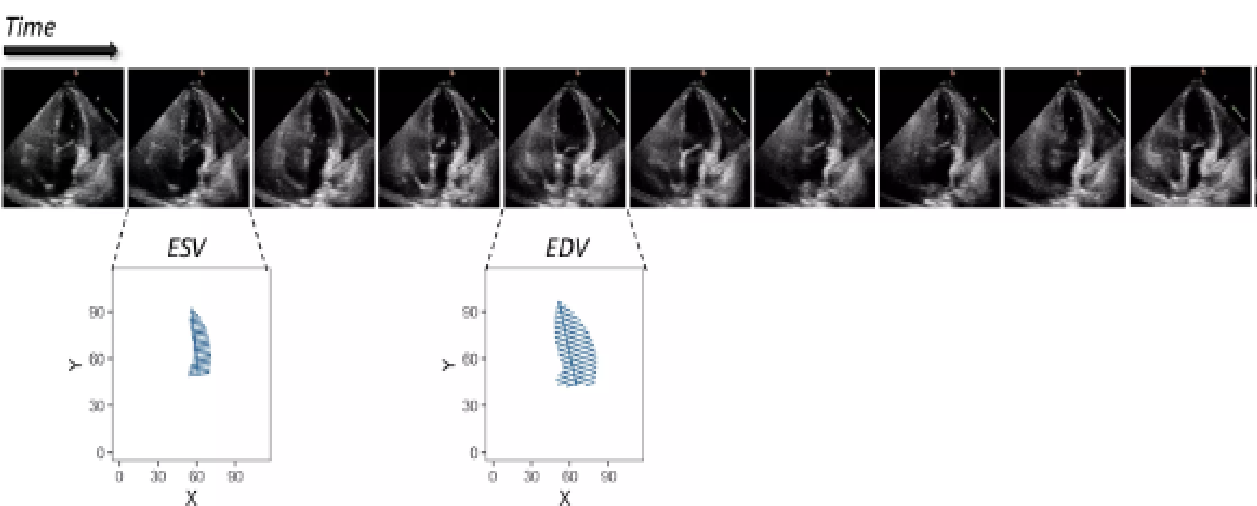
\includegraphics[width=1\linewidth]{capitulos//figuras/saidadoeco.png}
\caption{Frames representativos do ciclo cardíaco demonstrando o volume diastólico final e o volume sistólico final, usados para o cálculo da fração de ejeção de \textcite{Ouyang2020}.}
\label{fig:card}
\end{figure}


\section{A ultrasonografia e o ecocardiograma}
\label{sec:A ultra sonografia e o ecocardiograma}

A ecografia utiliza ondas sonoras do tipo ultrassônicas para criar imagens de estruturas internas do corpo humano \cite{9781496321282}. Na física, o termo "ultra-som" se aplica a toda energia acústica com frequência acima da audição humana (20.000 hertz ou 20 kilohertz) \cite{Carovac2011}. No diagnóstico médico, o ultrassom é usado como pulsos com frequência entre 3 e 10 MHz \cite{velavan}.

Essas ondas sonoras, quando utilizadas em ecografia, são caracterizadas por parâmetros essenciais que descrevem sua natureza. Estes incluem o comprimento de onda ($\Lambda$), que representa o comprimento da onda em metros, a frequência (\textit{f}), medida em Hertz, e a velocidade do ultrassom, que é aproximadamente 1540 m/s nos tecidos moles (v) \cite{Carovac2011}. O relacionamento entre a frequência (f), a velocidade e o comprimento de onda ($\lambda$) pode ser descrito pela Equação \eqref{eq:relacao}.

\begin{equation}
v = f \lambda
\label{eq:relacao}
\end{equation}


No contexto da ecografia, é importante ressaltar que as ondas de ultrassom são ondas mecânicas que requerem um meio físico para sua propagação \cite{Humphrey2007}. A complexa estrutura dos tecidos humanos torna-os heterogêneos, permitindo a observação de fenômenos como reflexão, refração e espalhamento das ondas sonoras\cite{velavan}.

 A formação de imagens por ultrassom é um processo  que se baseia na habilidade de mapear o nível de som retroespalhado em tons de cinza \cite{49500}. Para compreender a física por trás das imagens de ultrassom, é essencial examinar o comportamento do feixe sonoro ao interagir com o meio \cite{Papalo2019}.

Em suma, a capacidade do ultrassom em gerar imagens está diretamente ligada à reflexão e ao espalhamento das ondas sonoras nos contornos dos órgãos e em tecidos heterogêneos, causado pelas diferenças na impedância acústica \cite{Papalo2019}. Esse fenômeno permite a visualização de estruturas subcutâneas no corpo, incluindo tendões, músculos, articulações, vasos sanguíneos e órgãos internos, tornando possível a detecção de patologias ou lesões \cite{Papalo2019}.

 O ultrassom utilizado na área médica é gerado em materiais cristalinos especiais que, quando eletricamente excitados, têm a capacidade de vibrar em frequências extremamente altas, da ordem de milhões de vibrações por segundo. Os dispositivos que produzem e detectam o ultrassom são denominados transdutores \cite{ISBN9241592990}.

Os transdutores utilizados na ultrassonografia são fabricados a partir de materiais piezoelétricos. Esses materiais reagem à aplicação de uma diferença de potencial nos eletrodos de sua superfície, gerando uma deformação mecânica direcionada. Curiosamente, esse fenômeno pode ser observado de maneira inversa, onde a aplicação de uma força mecânica na superfície do material resulta na geração de uma voltagem nos eletrodos \cite{biscegli_2003}.


Na área médica, o transdutor de ultrassom, também conhecido como sonda ecoscópica, é um dispositivo inserido no corpo do paciente que contém um ou mais transdutores de ultrassom, conforme explicado por \textcite{Carovac2011}. A aplicação do ultrassom envolve uma variedade de tipos de transdutores, e a escolha do transdutor a ser utilizado depende do órgão ou tecido específico que será examinado, como destacado por \textcite{ufersa}. Os principais tipos de transdutores incluem o transdutor curvo ou convexo, que é usado em exames de órgãos internos como fígado, vesícula biliar, rins, feto, útero, ovários e coração; o transdutor linear, destinado a exames de órgãos externos e superficiais, incluindo tireoide, mamas, testículos, músculos, tendões e pele; o transdutor endocavitário, adequado para exames de órgãos internos através das vias naturais do corpo (esôfago, vagina, reto) ou durante cirurgias abertas ou fechadas; o transdutor setorial, usado principalmente para facilitar o exame de órgãos internos, como o coração e o cérebro; e transdutores especiais que utilizam tecnologias adicionais, como volumétrica e matricial, para obter imagens especiais, como 3D/4D e biplanares.


Os sinais elétricos produzidos pelos cristais piezoelétricos do transdutor são enviados a um amplificador e demonstrados no monitor com intensidades proporcionais à sua energia, permitindo que sejam decodificados por diferentes modos como o modo-A, modo-B e modo-M . O modo A do ultrassom consiste em uma imagem unidimensional exibida como uma série de picos verticais, que correspondem à profundidade das estruturas encontradas nos diferentes tecidos. A distância entre os picos ecoados pode ser calculada dividindo-se a velocidade do ultrassom no tecido (1540 m/s) pela metade do tempo decorrido, embora forneça poucas informações sobre a relação espacial das estruturas fotografadas. O modo B, amplamente utilizado na medicina, opera com vários cristais no transdutor que são acionados em sequência, realizando uma varredura de feixes de ultrassom que formam uma imagem bidimensional. Já o modo M é produzido por um único feixe em uma varredura de ultrassom para produzir uma imagem que exibe sinais de movimento, onde o movimento de uma estrutura, como uma válvula cardíaca, pode ser representado de maneira ondulatória \cite{ufersa}.

\section{Ecocardiograma}
\label{sec:Ecocardiograma}

A ultrassonografia cardíaca, também conhecida como ecocardiograma, é um dos exames mais empregados no diagnóstico de doenças cardíacas devido à sua natureza não invasiva, custo acessível e ampla disponibilidade. Na prática clínica, a ecocardiografia desempenha um papel fundamental na avaliação de cardiopatias, determinação do tamanho das câmaras cardíacas, avaliação de massas ventriculares, diagnóstico de valvopatias e análise da hemodinâmica do coração \cite{8520425232}.

\textcite{Mitchell2019-br} explica que para a aquisição de imagens bidimensionais do coração transtorácico, são definidas nomenclaturas que define planos, visões e manobras de varredura para a obtenção de imagens ecocardiográficas conforme Figura \ref{fig:planos}. Os movimentos do transdutor são descritos em relação aos eixos anterior, posterior, superior, inferior, lateral e medial. Todos os transdutores possuem uma marcação que determina a orientação. As janelas de varredura consideradas incluem paraesternal (localização do transdutor próximo ao esterno no peito), apical (localização do transdutor abaixo da mama esquerda, perto do ápice do coração), subcostal (posicionamento do transdutor abaixo do esterno, melhor obtido com o paciente deitado de costas) e supraesternal (posicionamento do transdutor acima do esterno, mostrando o arco aórtico) como descrito na Figura \ref{fig:planos2} . 

Para a aquisição das janelas paraesternal e apical, o paciente é posicionado em decúbito lateral esquerdo. Na projeção paraesternal em eixo longo (PLAX), a marcação do índice de localização aponta para o ombro direito do paciente. Já na visão paraesternal em eixo curto (PSAX), a marcação aponta para o ombro esquerdo, proporcionando imagens em plano axial. A janela apical é localizada abaixo da mama esquerda, permitindo a visualização do ápice cardíaco\cite{Mitchell2019-br} .

 
 \begin{figure}[H]
   \centering
   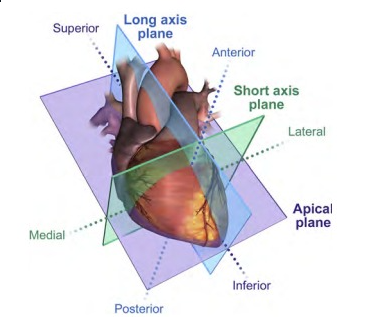
\includegraphics[width=0.6\linewidth]{capitulos/figuras/planos.png}
   \caption{Nomenclaturas que define planos, visões e manobras de varredura para a obtenção de imagens ecocardiográficas. Retirado de \textcite{Mitchell2019-br}}
   \label{fig:planos}
\end{figure}

 \begin{figure}[H]
   \centering
   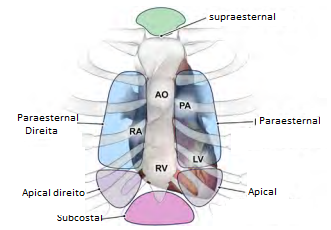
\includegraphics[width=0.6\linewidth]{capitulos/figuras/planos2.png}
   \caption{Nomenclaturas que define janelas ecocardiográficas. Imagens de \textcite{Mitchell2019-br}.}
   \label{fig:planos2}
\end{figure}

No contexto desta dissertação, a avaliação do tamanho do ventrículo esquerdo (VE) desempenha um papel crucial na análise da função cardíaca usando ecocardiograma. Essa avaliação envolve a utilização de parâmetros que incluem dimensões lineares internas e volumes do VE, obtidos tipicamente no final da diástole e da sístole. 
Esses parâmetros são essenciais para determinar a fração de ejeção cardíaca, um indicador crítico da função cardíaca. As medidas lineares, preferencialmente obtidas no corte paraesternal de eixo longo representados na Figura \ref{fig:parasternal}, requerem cuidadosa colocação do cursor eletrônico para evitar secções oblíquas do ventrículo, enquanto as medidas volumétricas, baseadas em traçados das interfaces entre o miocárdio e a cavidade, são mais precisas do que os cálculos lineares que assumem uma forma geométrica fixa do VE \cite{Lang2015}. 

\begin{figure}[H]
\centering
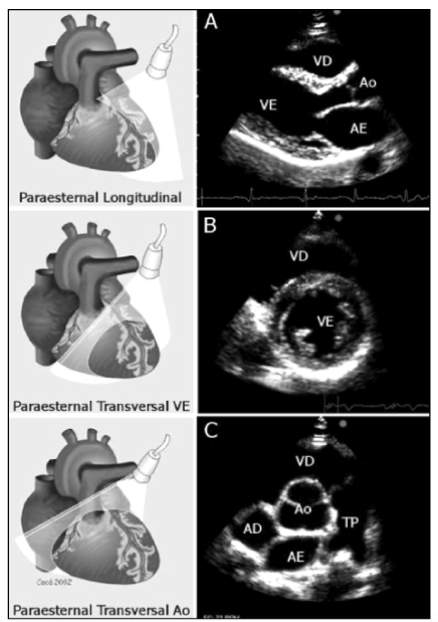
\includegraphics[width=0.6\linewidth]{capitulos/figuras/paraesternalC.png}
\caption{Corte Paraesternal de Eixo Longo do Ventrículo Esquerdo, imagem de \textcite{Silva2004}.}
\label{fig:parasternal}
\end{figure}

\textcite{Lang2015} indica que para medições volumétricas precisas, é aconselhável obter volumes a partir dos cortes apicais quatro e duas câmaras, maximizando as áreas do VE e evitando o encurtamento do ventrículo esquerdo, o que poderia resultar em uma subestimação do volume.

\begin{figure}[H]
\centering
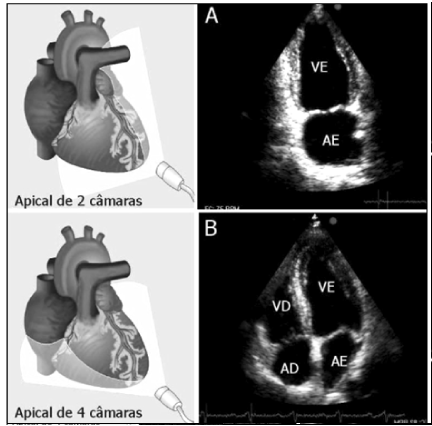
\includegraphics[width=0.6\linewidth]{capitulos/figuras/Apical.png}
\caption{Representação da técnica de Simpson para ecocardiograma apical de 4 câmaras e de 2 câmaras \textcite{Lang2015} }
\label{fig:apical}
\end{figure}

A estimativa do volume do ventrículo esquerdo (VE) pode ser adquirida tanto por meio da ecocardiografia bidimensional (E2D) quanto da ecocardiografia tridimensional (E3D). No contexto da E2D, o método predominante para calcular o volume do VE é o conhecido método biplanar da soma de discos conforme Figura \ref{fig:figsimpsom}.

\begin{figure}[H]
\centering
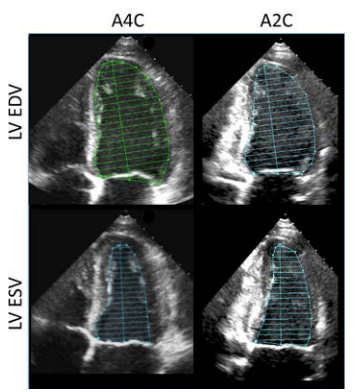
\includegraphics[width=0.3\linewidth]{capitulos/figuras/simpsons.png}
\caption{Representação da técnica de Simpson para ecocardiograma apical de 4 câmaras e de 2 câmaras, \textcite{Lang2015})}
\label{fig:figsimpsom}
\end{figure}


Como alternativa viável  o método área-comprimento na Figura \ref{fig:figcomprimento}, o qual presume que o VE possui uma forma semelhante à de um projétil. Nesse método, a área da seção transversal do VE no terço médio do corte paraesternal de eixo-curto é calculada, e o comprimento do ventrículo é estimado a partir do ponto médio do plano anular no corte apical de quatro câmaras, ressaltando que a suposição da forma de projétil nem sempre é precisa, esse método é mostrado na Figura\ref{fig:3d}.


\begin{figure}[H]
\centering
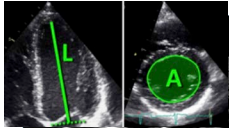
\includegraphics[width=0.3\linewidth]{capitulos/figuras/comprimento.png}
\caption{Representação da técnica do método área-comprimento, retirado de \textcite{Lang2015}.}
\label{fig:figcomprimento}
\end{figure}

\begin{figure}[H]
\centering
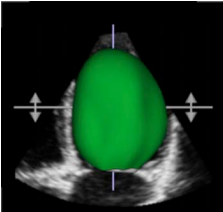
\includegraphics[width=0.3\linewidth]{capitulos/figuras/3d.png}
\caption{Representação da técnica por medição do volume por meio da ecocardiografia tridimensional (E3D) por \textcite{Lang2015}}
\label{fig:3d}
\end{figure}


 Os valores normais para parâmetros ecocardiográficos 2D relacionados ao tamanho do ventrículo esquerdo e sua função, segmentados de acordo com o sexo dos pacientes. Esses valores, detalhados na Tabela \ref{tab:echoparams}, incluem médias e variações de dois desvios padrão (2SD) para cada parâmetro, tanto para homens quanto para mulheres. As variações de 2SD fornecem um intervalo importante, indicando onde se espera encontrar aproximadamente 95\% das medições para uma distribuição normal dos dados.

\begin{table}[htbp]
\centering
\small % Diminui a fonte da tabela
\caption{Parâmetros Ecocardiográficos}
\label{tab:echoparams}
\begin{tabular}{lcccc}
\toprule
Parâmetro & \multicolumn{2}{c}{Homens} & \multicolumn{2}{c}{Mulheres} \\
\cmidrule(lr){2-3} \cmidrule(lr){4-5}
& Média ± DP & Variação 2DP & Média ± DP & Variação 2DP \\
\midrule
Dimensão Diastólica Interna (mm) & 50.2 ± 4.1 & 42.0-58.4 & 45.0 ± 3.6 & 37.8-52.2 \\
Dimensão Sistólica Interna (mm) & 32.4 ± 3.7 & 25.0-39.8 & 28.2 ± 3.3 & 21.6-34.8 \\
Volume Diastólico Final (mL) & 106 ± 22 & 62-150 & 76 ± 15 & 46-106 \\
Volume Sistólico Final (mL) & 41 ± 10 & 21-61 & 28 ± 7 & 14-42 \\
Volume Diastólico Final (mL/m²) & 54 ± 10 & 34-74 & 45 ± 8 & 29-61 \\
Volume Sistólico Final (mL/m²) & 21 ± 5 & 11-31 & 16 ± 4 & 8-24 \\
Fração de Ejeção (\%) & 62 ± 5 & 52-72 & 64 ± 5 & 54-74 \\
\bottomrule
\end{tabular}
\end{table}



A Tabela \ref{tab:severidade_ve} mostra as faixas de valores normais e pontos de corte de graus de severidade para a fração de ejeção do ventrículo esquerdo, derivados do ecocardiograma 2DE, segmentados por sexo. Essas faixas são úteis na avaliação da função cardíaca e na identificação de anomalias, permitindo que profissionais de saúde e pesquisadores determinem o grau de severidade de possíveis problemas cardíacos em pacientes do sexo masculino e feminino \cite{Lang2015}.

\begin{table}[htbp]
\centering
\caption{Faixa de Valores Normais e Pontos de Corte de Graus de Severidade para a Fração de Ejeção do Ventrículo Esquerdo Derivados do 2DE.}
\label{tab:severidade_ve}
\begin{tabular}{lcc}
\toprule
\textbf{Parâmetros} & \textbf{Homem} & \textbf{Mulher} \\
\midrule
Faixa Levemente normal & 52 - 72 & 54 - 74 \\
Anormal & 41 - 51 & 41 - 53 \\
Moderadamente anormal & 30 - 40 & 30 - 40 \\
Gravemente anormal & <30 & <30 \\
\bottomrule
\end{tabular}
\end{table}

\section{Redes neurais artificiais}
\label{sec:Redes neurais}

Segundo \textcite{haykin2001redes}, as Redes Neurais Artificiais (RNAs) são sistemas de processamento paralelos compostos por unidades simples, capazes de armazenar conhecimento e utilizá-lo no futuro. Embora haja ainda muito a ser compreendido sobre o funcionamento neurofisiológico dos neurônios e suas conexões, as RNAs compartilham características fundamentais com o cérebro. Elas extraem conhecimento do ambiente por meio de um processo de aprendizagem ou treinamento, e os pesos sinápticos, que representam as conexões entre os neurônios, são utilizados para armazenar o conhecimento adquirido.

Essas semelhanças entre as RNAs e o cérebro destacam-se em sua capacidade de adquirir conhecimento do ambiente através de aprendizagem e treinamento, além do armazenamento desse conhecimento nos pesos sinápticos. No entanto, é importante reconhecer que a fidelidade desses modelos em relação à fisiologia real ainda é limitada devido à complexidade do funcionamento neurofisiológico. A pesquisa em RNAs envolve diversas disciplinas, como neurofisiologia, psicologia, física, computação, engenharia e estatística, permitindo uma abordagem multidisciplinar para explorar todo o potencial dessas redes neurais artificiais \cite{haykin2001redes}.


\textcite{haykin2001redes} descreve que as redes neurais artificiais são construídas com base em modelos matemáticos inspirados pela cognição humana e pela neurobiologia, contendo vários pressupostos essenciais. Primeiramente, assumimos que o processamento da informação ocorre por meio de elementos chamados neurônios. Cada neurônio recebe sinais de entrada, realiza cálculos internos e gera um sinal de saída, sendo estes neurônios artificiais análogos aos neurônios biológicos encontrados no cérebro humano. Além disso, os neurônios nas redes neurais artificiais são interconectados por meio de conexões que permitem a transmissão dos sinais de um neurônio para outro, com cada conexão possuindo um peso associado que representa a importância relativa dessa conexão na transmissão do sinal. Os pesos sinápticos são ajustados durante o processo de aprendizado para otimizar o desempenho da rede. No que se refere à transmissão do sinal, em uma rede neural típica, a transmissão de sinal de um neurônio para o próximo é ponderada pelo peso sináptico associado à conexão entre eles, determinando a contribuição relativa desse sinal na ativação do neurônio de destino. Ou seja, alguns sinais podem ter mais influência do que outros com base nos pesos sinápticos correspondentes. Cada neurônio, ou unidade, em uma rede neural artificial possui também uma função de ativação, que recebe a soma ponderada dos sinais de entrada e produz a saída do neurônio. Geralmente, as funções de ativação são não-lineares, permitindo que a rede modele relações complexas entre os dados.

Incorporando todos os elementos mencionados por \textcite{CHAI2021100134}, as redes neurais artificiais demonstram uma  habilidade para aprender e discernir padrões  a partir dos dados de entrada. Esta capacidade de processar informações multifacetadas e adaptar-se de forma autônoma as torna extremamente valiosas em diversas aplicações, incluindo classificação, previsão e reconhecimento de padrões. Devido a essa versatilidade, elas são essenciais em campos variados, como visão computacional, processamento de linguagem natural (NLP), reconhecimento de voz e de vídeo, além de serem amplamente utilizadas no setor financeiro e bancário.

No centro dessa revolução tecnológica, destacam-se várias arquiteturas de rede neural, cada uma com características e aplicações específicas na visão computacional. Entre as mais proeminentes estão as Redes Neurais Convolucionais (CNNs), Redes Neurais Recorrentes (RNNs), Redes Adversárias Gerativas (GANs), Redes de Função de Base Radial (RBFNs), Perceptrons Multicamadas (MLPs), Mapas Auto-Organizáveis (SOMs), Redes de Crenças Profundas (DBNs), Máquinas Boltzmann Restritas (RBMs) e Autoencoders. Cada uma dessas arquiteturas oferece abordagens únicas e especializadas, contribuindo significativamente para os avanços e desafios da visão computacional \cite{CHAI2021100134}.

Neste contexto, o próximo Capítulo, \ref{Revisão bibliográfica}, explorará a aplicação de redes neurais profundas na avaliação da função cardíaca utilizando vídeos de ecocardiograma, analisando e discutindo trabalhos relevantes nesse campo. 



\pagestyle{ruledheader} %inclui novo capítulo
\chapter{Revisão bibliográfica}
\label{Revisão bibliográfica}

Neste Capítulo, exploramos a aplicação de redes neurais profundas na avaliação da função cardíaca utilizando vídeos de ecocardiograma, com o objetivo de analisar e discutir trabalhos relevantes nesse campo.  A Seção \ref{Revisão Sistemática da Literatura} descreve a metodologia de Revisão Sistemática da Literatura (SLR), onde apresentamos uma visão geral das estratégias utilizadas para a seleção dos trabalhos pertinentes. Na Seção \ref{Estudos selecionados} descreve os aspectos teóricos das redes neurais profundas empregadas nos estudos escolhidos, seguidos por uma apresentação e discussão criteriosa dos trabalhos relacionados a essa redes neurais, organizados por temas relevantes para a área de interesse deste trabalho. Esta Seção é estruturada de forma a proporcionar um aprofundamento teórico nas tecnologias de redes neurais, enquanto simultaneamente contextualiza cada estudo selecionado dentro do âmbito da avaliação da função cardíaca por meio de ecocardiograma.
 Em cada bloco temático desta Seção, após a apresentação dos trabalhos, incluímos uma discussão detalhada, examinando a metodologia, os resultados e as contribuições de cada pesquisa para o campo da avaliação cardíaca. Essas discussões são integradas ao final de cada tema, proporcionando uma análise abrangente que destaca tanto os avanços técnicos quanto as implicações práticas desses estudos no contexto mais amplo da avaliação cardíaca utilizando tecnologias de aprendizado profundo. Através desta abordagem, o Capítulo oferece uma perspectiva completa sobre como as redes neurais profundas estão sendo utilizadas para inovar e melhorar a precisão da avaliação cardíaca em ecocardiogramas.

\section{Revisão Sistemática da Literatura}
\label{Revisão Sistemática da Literatura}

O protocolo de revisão sistemática da literatura, estabelecido seguindo as orientações de \cite{kitchenham2009systematic}, é um estudo que tem como objetivo fornecer uma abordagem imparcial, objetiva e sistemática para responder a questões específicas de pesquisa, tópicos de uma área ou fenômenos de interesse. Esses fenômenos, conhecidos como estudos primários, são analisados e sintetizados dentro do contexto da revisão, permitindo uma compreensão aprofundada e estruturada do campo em questão.

A Revisão Sistemática da Literatura (SLR) constitui um método meticuloso e estruturado, essencial para compreender as tendências e os avanços em campos específicos, como a avaliação de imagens e vídeos de ecocardiograma usando abordagens de Deep Learning. Este método, pautado pelas diretrizes de \textcite{kitchenham2009systematic}, divide-se em três fases fundamentais: planejamento, condução e relatório. Na fase de planejamento, a ênfase recai sobre a definição clara das questões de pesquisa. Este passo é crucial pois as questões moldam o escopo da revisão, direcionando a busca e análise dos estudos. As questões devem ser precisas e relevantes, refletindo as necessidades de informação no campo de estudo. A formulação destas questões é descrita na Seção \ref{Questões de pesquisa} e serve como a espinha dorsal para as etapas subsequentes. Seguindo para a fase de condução, detalhada na Seção \ref{Abordagem de pesquisa}, o processo se volta para a identificação e seleção de estudos relevantes. Esta etapa é caracterizada por uma busca sistemática em bases de dados e literatura científica, utilizando critérios de inclusão e exclusão. A condução é uma fase detalhada, garantindo que apenas os estudos mais pertinentes e de alta qualidade sejam considerados para análise. Por fim, a fase de relatório trata da síntese e apresentação dos resultados encontrados. Aqui, os estudos selecionados são avaliados, analisados e os achados são relatados de maneira estruturada e coerente. A qualidade dos estudos incluídos é avaliada, conforme descrito na subSeção \ref{Avaliação de qualidade}.

\subsection{Questões de pesquisa}
\label{Questões de pesquisa}

Esta revisão sistemática da literatura teve como objetivo apresentar os estudos que foram publicados na área de avaliação de imagens e vídeos de ecocardiograma  usando abordagens de \textit{Deep Learning} . As questões de pesquisa abordadas por esta pesquisa são:

Questão 1 (Q1) Em quais tipos de ecocardiograma a IA foi aplicada ?

Questão 2 (Q2) - Quais estruturas do coração o artigo trata?

Questão 3 (Q3) - Quais marcadores ou doença são avaliado?

Questão 4 (Q4) - Quais modelos de \textit{Machine Learning}  ou \textit{Deep Learning}  vêm sendo mais utilizados para avaliação do coração?

Questão 5 (Q5) - Quais conjuntos de dados são utilizadas para treinar e testar os algoritmos de \textit{Machine Learning}/\textit{Deep Learning} ?

Questão 6 (Q6) - Quais são os parâmetros de avaliação e abordagens utilizadas para modelos de DL/ML  em ecocardiograma foi aplicada para apoiar a decisão médica?

\subsection {Abordagem de pesquisa}
\label{Abordagem de pesquisa}

Uma abordagem sistemática foi adotada para restringir os resultados da pesquisa aos artigos que estão diretamente relacionados ao escopo do SLR. Para identificar contribuições relacionadas, motores de busca como Science Direct , IEEE Explore, PubMed  e Google Scholar foram consultados para artigos contendo (“machine learning” OR “deep learning”) AND (“Echocardiography”)  no título e resumo. 

A última atualização dos documentos incluídos foi em 1º de setembro de 2022.

Todos os resultados foram processados e as strings de busca acima mencionadas resultaram em um total de 436 estudos.

\subsection {Critério de seleção}
\label{Critério de seleção}

Nesta etapa serão definidos os critérios de seleção/inclusão e exclusão para definir quais artigos passarão para a próxima etapa da revisão. Os critérios devem ser definidos a partir das questões de pesquisa. Os resultados da pesquisa de diferentes bancos de dados foram adicionados a uma planilha e verificados de acordo com os critérios de seleção. Para que um estudo seja incluído, todos os critérios de inclusão devem ser verdadeiros e os critérios de exclusão devem ser falsos \cite{kitchenham2009systematic}.

Todos os estudos extraídos que pudessem responder às questões de pesquisa foram considerados potencialmente relevantes e selecionados para passar pelos critérios de inclusão e exclusão apresentados a seguir.

A publicação é sobre o uso de Deep Learning ou Machine Learning para análises de vídeos e imagens em ecocardiograma. 

A publicação é um estudo primário. (Estudos primários são investigações originais que envolvem a coleta e análise de dados diretamente dos experimentos ou observações, sem depender de dados já publicados por outros estudos. Eles são a fonte principal de novas informações científicas.)

O artigo foi publicado após o ano de 2019. 

Os critérios de exclusão utilizados foram os seguintes.

1: A publicação não está relacionada ao Deep Learning ou Machine learning para  analises de vídeos e imagens em ecocardiograma.

2: A publicação é duplicada ou recuperada de outro banco de dados.

3: O texto completo do estudo não está disponível.

4: O estudo não está publicado na língua inglesa


Após a exclusão dos registros duplicados (n = 32), os critérios de seleção foram aplicados aos demais registros (n = 404). Assim, um total de 113 artigos de texto completo foram avaliados para elegibilidade. Para a seleção dos artigos finais, foram considerados artigos publicados nos últimos três anos. 

\subsection {Avaliação de qualidade}
\label{Avaliação de qualidade}

O próximo passo no protocolo de revisão foi a execução da  avaliação da qualidade. \textcite{kitchenham2009systematic} define que esse passo tem como objetivo avaliar melhor os estudos incluídos e remover estudos que não se encaixam no objetivo desta revisão ou que não descrevem os detalhes que são importantes para esta revisão com detalhes suficientes. 

Com esse objetivo, foram estabelecidos os  seguintes critérios de avaliação:

1: O objetivo da pesquisa está claramente descrito?

2: O artigo possui citações? Se sim são citações é > 5 ou > 15?

3: Os autores descreveram as limitações do estudo?

4: O estudo deixa claro quais foram as oportunidades identificadas?

5: O estudo conseguiu resolver o ou propor solução para o problema proposto?

Para execução desta etapa, os artigos foram analisados para responder aos critérios de avaliações propostos. pode ser obtido 1 ponto se o critério for atendido, ou meio ponto se for parcialmente atendido. Isso deu uma pontuação de qualidade entre 0 e 5 para cada estudo. Artigos com pontuação acima ou iguais a 4,5 foram incluídos nesta revisão.

O fluxograma das etapas iterativas de seleção dos estudos foi elaborado a partir
da metodologia e está apresentado na Figura \ref{fig:fluxoslr}. A Tabela \ref{tab:trabalhos} apresenta os artigos selecionados para leitura na íntegra.

\begin{figure}[H]
   \centering
   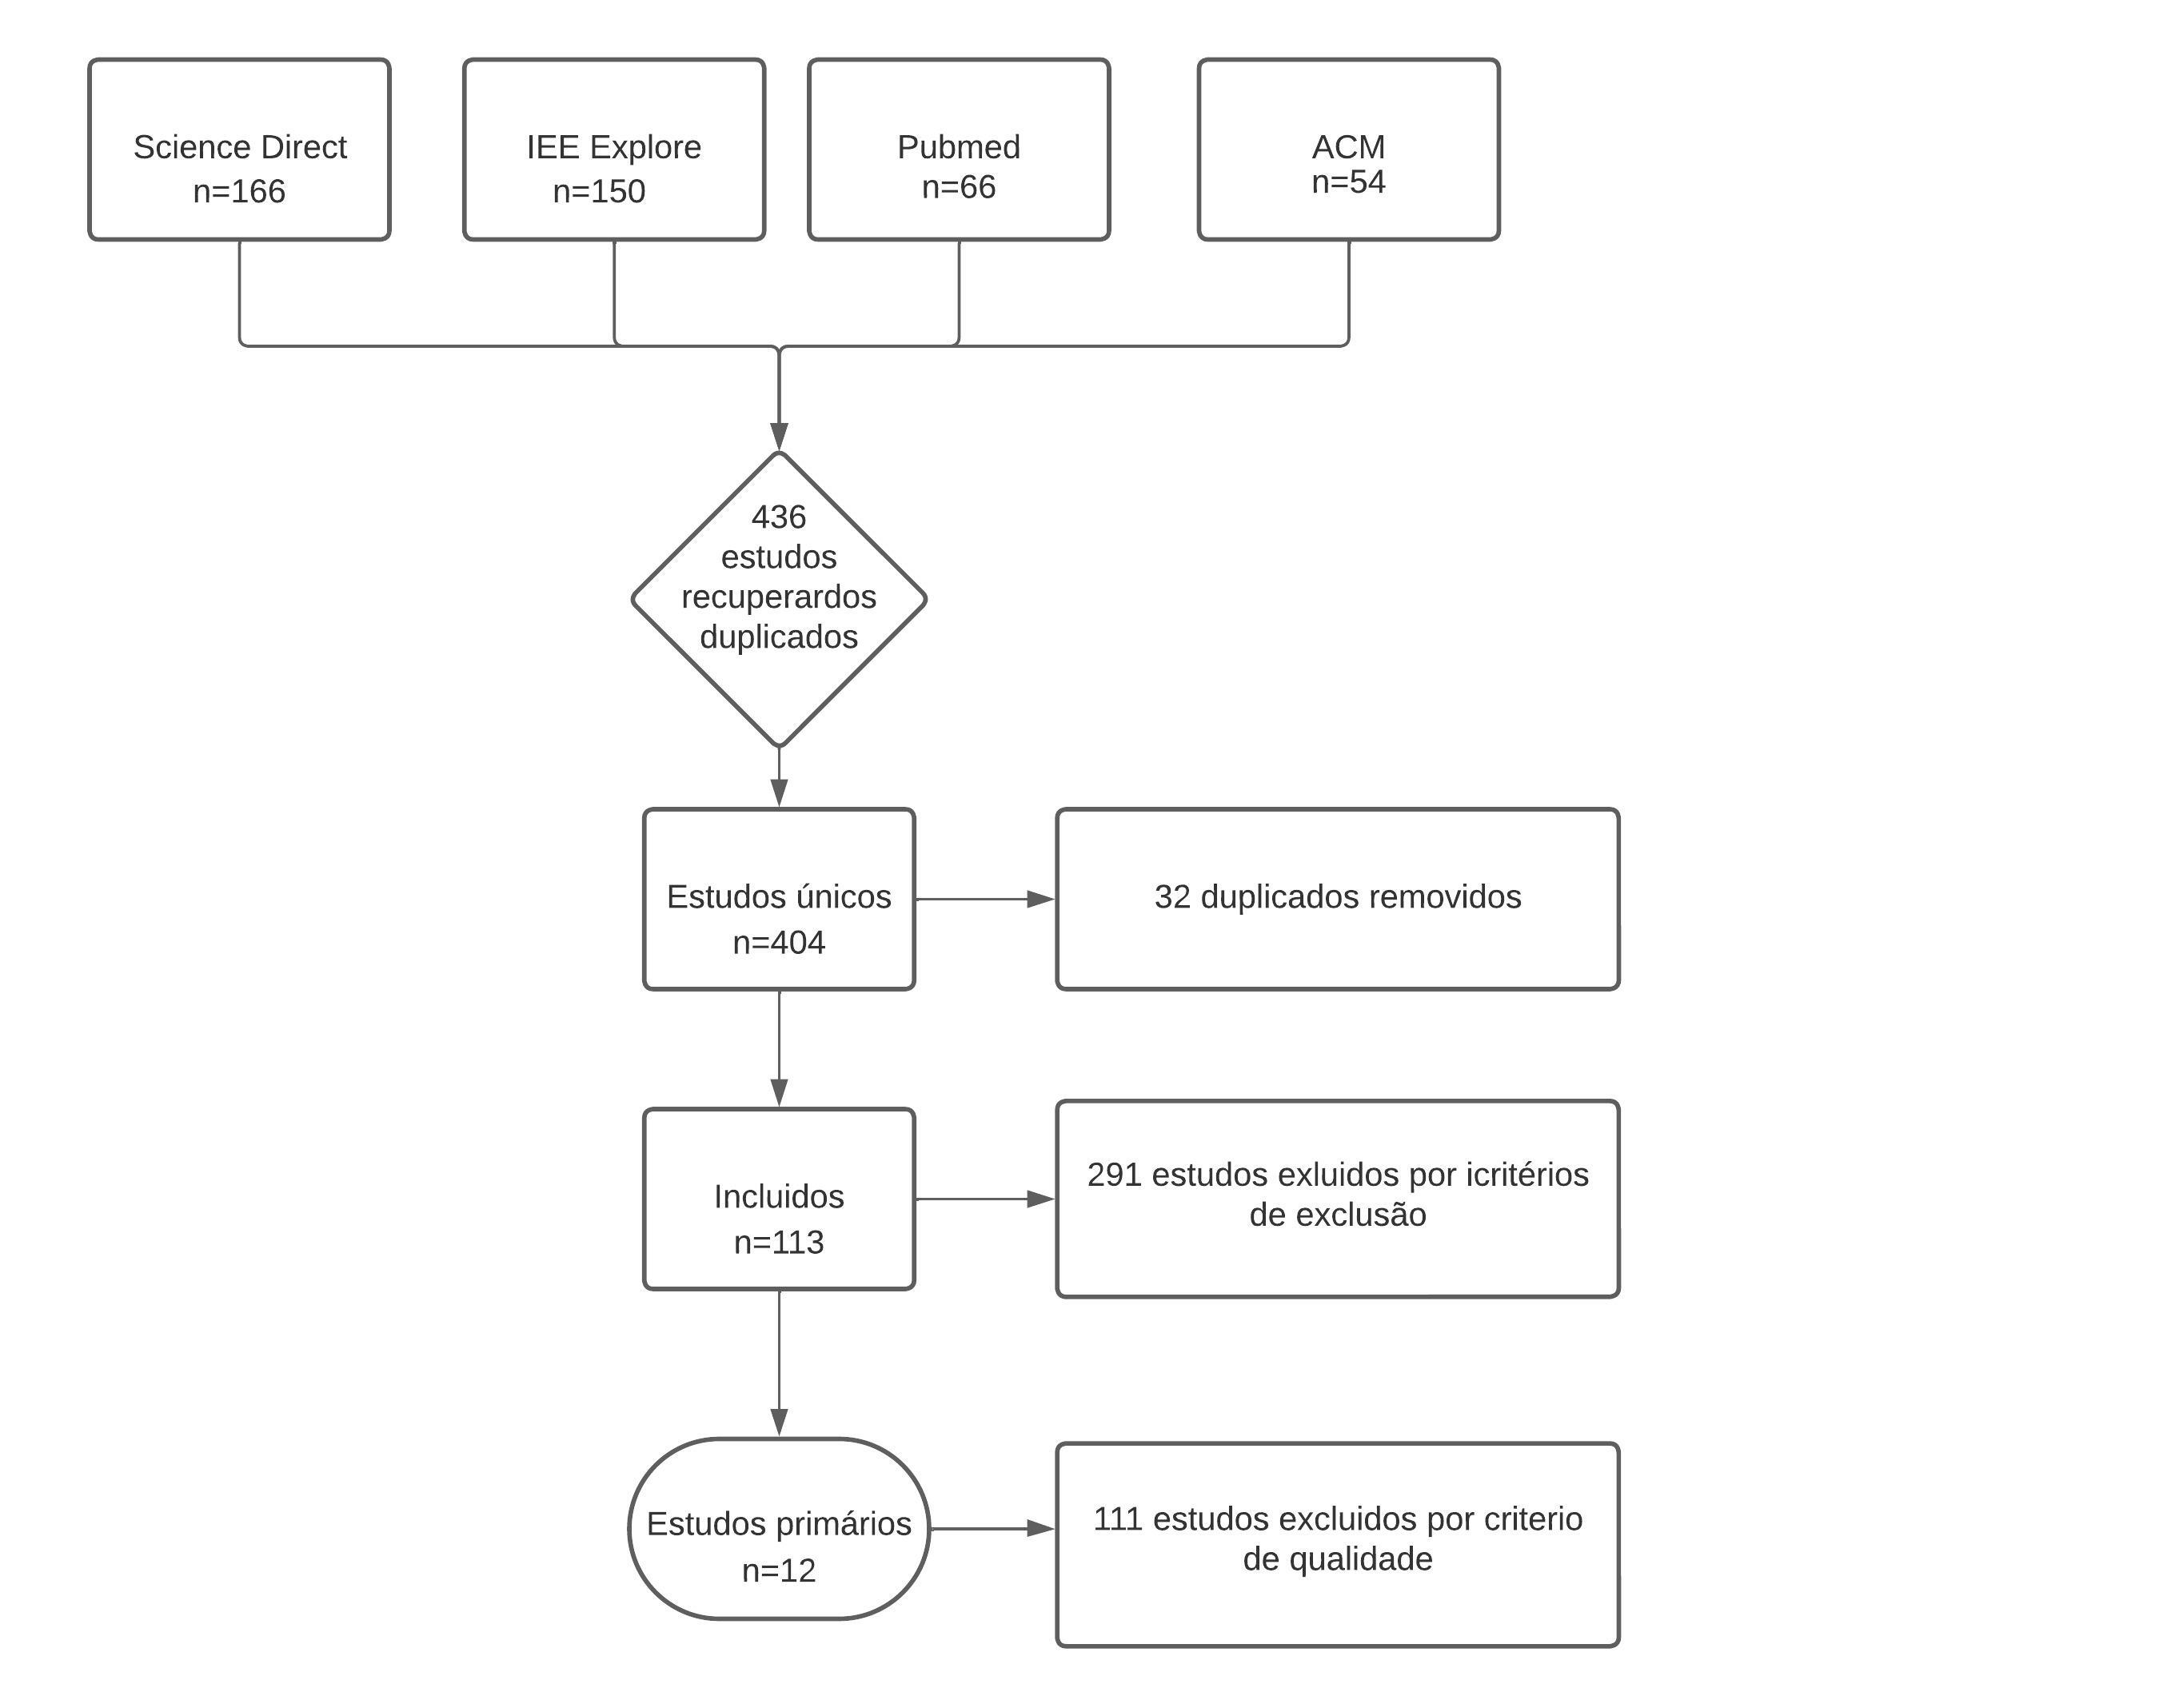
\includegraphics[width=0.8\linewidth]{capitulos/figuras/diagrama_slr.jpeg}
   \caption{Etapas da revisão sistemática da literatura.}
   \label{fig:fluxoslr}
\end{figure}

\begin{table}[!ht]
\begin{center}
\caption{Tabela de artigos selecionados}
\label{tab:trabalhos}
\resizebox{\textwidth}{!}{
\begin{tabular}{c c}
\hline
\textbf{Artigo} & \textbf{Algoritmo} \\
\hline
% 1 trabalho
\textcite{LIU2021101873} & Rede Neural Convolucional (CNN) com uma rede de atenção local \\
% 2 trabalho
\textcite{9648607} & Rede Neural Convolucional (CNN) e Rede neural Bayesiana \\
% 3 trabalho
\textcite{9335592} & Rede Neural Convolucional (CNN) \\
% 4 trabalho
\textcite{10.1001/jamacardio.2021.6059} & Rede Neural Convolucional (CNN) \\
% 5 trabalho
\textcite{Ouyang2020} & Rede Neural Convolucional (CNN) \\
% 6 trabalho
\textcite{Sun2021} & Rede Neural Convolucional (CNN) \\
% 7 trabalho
\textcite{corinzia2020neural} & Filtragem Colaborativa Neural \\
% 8 trabalho
\textcite{DONG2020101638} & AtlasNet \\
% 9 trabalho
\textcite{8931542} & Rede Neural Convolucional (CNN) \\
% 10 trabalho
\textcite{8649738} & Rede Neural Convolucional (CNN) com Arquitetura Encoder-Decoder \\
% 11 trabalho
\textcite{8586941} & DenseNet, ResNet e LSTM Bidirecional \\
% 12 trabalho
\textcite{Reynald} & Rede neural transformes e ResnetAE Encoder-Decoder\\
\hline
\end{tabular}}
\end{center}
\end{table}

\section{Estudos selecionados}
\label{Estudos selecionados}

Nesta Seção, a Seção \ref{subsec:Redes neurais convolucionais} será dedicada a uma análise detalhada dos conceitos fundamentais das redes neurais artificiais convolucionais, com um enfoque especial em sua aplicação na análise de imagens de ecocardiogramas. Esta Seção explorará a estrutura, as funcionalidades e as implicações práticas das redes convolucionais, fornecendo um entendimento aprofundado de como essas redes processam e interpretam imagens. Além disso, será apresentada uma revisão de trabalhos significativos que empregam a CNN na análise de ecocardiogramas, destacando avanços recentes e como esses estudos contribuem para o campo da imagem médica. Após delinear esses aspectos e trabalhos relacionados, a discussão evoluirá para a próxima subSeção  \ref{subsec:Redes neurais transformers}, na qual serão introduzidos os conceitos de redes transformadoras e trabalhos relacionados, abrindo um novo horizonte no contexto do processamento avançado de imagens médicas. 

\section{Redes neurais convolucionais}
\label{subsec:Redes neurais convolucionais}

%!explicação Redes neurais convolucionais


O primeiro grupo de arquitetura nos trabalhos selecionados são as redes neurais convolucionais. \textcite{CHAI2021100134} define a CNN como uma estrutura composta por camadas convolucionais, de pooling e totalmente conectadas. As camadas convolucionais se destacam por utilizar vários núcleos para processar a imagem inteira e os mapas de características intermediários, resultando na formação de diversos mapas de características.

Em um modelo de CNN, a entrada X de cada camada é estruturada em três dimensões: altura (a), largura (l) e profundidade (p), sendo que a altura é igual à largura. A profundidade, que também pode ser descrita como o número de canais, varia conforme o tipo de imagem; por exemplo, tem valor três em imagens RGB. Além disso, em cada camada convolucional, estão presentes vários núcleos ou filtros, identificados pela letra k, que também são tridimensionais, seguindo as mesmas dimensões de altura, largura e profundidade.

\textcite{Alzubaidi2021} explica as várias etapas e componentes da arquitetura de uma CNN. A camada convolucional, sendo o componente mais significativo da arquitetura, consiste em uma coleção de filtros convolucionais. Esses filtros são usados para convolucionar a imagem de entrada, que é expressa em métricas N-dimensionais, resultando na geração do mapa de características de saída. O \textit{kernel}, que se configura como uma matriz composta por uma série de valores numéricos discretos, conhecidos como pesos do \textit{kernel}, é inicialmente atribuído de forma aleatória. Existem diversas técnicas para essa inicialização, cada uma com características específicas. Conforme o treinamento avança, passando por várias \textit{epochs}, ocorre um processo de ajuste e refinamento desses pesos. Essa etapa é crucial, pois permite que o \textit{kernel} aprimore sua capacidade de identificar e extrair características relevantes dos dados de entrada, contribuindo significativamente para o processo de aprendizado da rede.

Na arquitetura de uma CNN, a operação convolucional é um processo central que difere das redes neurais tradicionais em sua abordagem de entrada de dados. Enquanto as redes neurais convencionais utilizam um formato vetorial para a entrada, as CNNs processam imagens multicanais, como as de canal único em escala de cinza ou as RGB de três canais. Para ilustrar essa operação, consideremos uma imagem em escala de cinza de 4 × 4 e um \textit{kernel} de 2 × 2 com pesos inicializados aleatoriamente. Durante a convolução, o \textit{kernel} desliza sobre a imagem, tanto horizontal quanto verticalmente, e em cada posição, o produto escalar entre a imagem e o \textit{kernel} é calculado. Esse cálculo envolve multiplicar e somar os valores correspondentes para gerar um valor escalar único, que compõe o mapa de características de saída. Este processo continua até que o \textit{kernel} não possa mais deslizar sobre a imagem.

Dois conceitos importantes na operação convolucional são o \textit{padding} e o \textit{stride}. O \textit{padding} refere-se à adição de pixels extras ao redor da borda da imagem de entrada, permitindo que o \textit{kernel} processe completamente todas as áreas da imagem, incluindo as bordas, evitando a perda de informações de borda. Isso é especialmente importante para manter o tamanho da imagem de entrada após a convolução. Por outro lado, o \textit{stride} define o tamanho do passo que o \textit{kernel} dá ao deslizar sobre a imagem. Um \textit{stride} de um, por exemplo, significa que o \textit{kernel} se move um pixel de cada vez, enquanto um \textit{stride} maior resulta em um salto de mais pixels e, consequentemente, um mapa de características com dimensões menores. A escolha do \textit{stride} e a aplicação de \textit{padding} são decisões estratégicas no design da CNN, pois influenciam diretamente na captura de características e no tamanho do mapa de características.

A camada de \textit{pooling} desempenha a função crucial de subamostrar os mapas de características que são gerados após as operações convolucionais. Este processo consiste em reduzir o tamanho dos mapas de características, criando versões menores, mas ainda preservando a maioria das informações dominantes. Antes de iniciar a operação de \textit{pooling}, tanto o \textit{stride} quanto o tamanho do \textit{kernel} são definidos. Existem vários métodos de \textit{pooling}, incluindo \textit{pooling} máximo, mínimo, médio, \textit{tree pooling}, \textit{gated pooling}, \textit{global average pooling} (GAP) e \textit{global max pooling}, sendo os métodos de \textit{pooling} máximo, mínimo e GAP os mais comuns. Apesar de sua importância na redução de dimensionalidade e na manutenção de características relevantes, a camada de \textit{pooling} pode às vezes diminuir o desempenho geral da CNN, pois, enquanto ajuda a determinar a presença de características específicas, pode não capturar sua localização exata, o que pode levar à perda de informações críticas para o modelo.

Em todas as redes neurais, inclusive as redes transformes que serão explicadas posteriormente, a função de ativação desempenha um papel fundamental, sendo responsável por transformar os dados de entrada em saída. Esta transformação envolve o cálculo de uma soma ponderada dos inputs de cada neurônio, adicionando-se o viés quando este é parte da estrutura do neurônio. A função de ativação determina a ativação ou não de um neurônio com base nesses valores de entrada, produzindo assim a saída correspondente. Em uma arquitetura de CNN, as camadas de ativação não-lineares são utilizadas após todas as camadas com pesos, conhecidas como camadas aprendíveis, que incluem as camadas totalmente conectadas (FC) e as camadas convolucionais. A natureza não-linear dessas camadas de ativação implica que o mapeamento de entrada para saída também será não-linear, permitindo que a CNN aprenda padrões mais complexos. Além disso, é crucial que a função de ativação possa ser diferenciada, uma característica extremamente importante para permitir que o erro de retro propagação seja utilizado no treinamento da rede.

\textcite{Alzubaidi2021} apresenta que diversas funções de ativação são empregadas nas CNNs, cada uma com características e equações matemáticas específicas. Entre elas estão a função Sigmoide, a função Tanh, a função ReLU e a função Leaky ReLU. A função Sigmoide aceita números reais como entrada e restringe a saída a valores entre zero e um. Sua curva é em forma de S e é matematicamente representada pela Equação \ref{eq:1}.

\begin{equation}
f(x)_{\text{sigm}} = \frac{1}{1 + e^{-x}}
\label{eq:1}
\end{equation}

A função Tanh, semelhante à Sigmoide em termos de aceitar números reais, limita a saída a valores entre -1 e 1, representada pela Equação \ref{eq:2}.

\begin{equation}
f(x)_{\text{tanh}} = \frac{e^x - e^{-x}}{e^x + e^{-x}}
\label{eq:2}
\end{equation}

A função ReLU, comumente utilizada no contexto das CNNs, transforma todos os valores de entrada em números positivos, sendo preferida devido à menor carga computacional. Sua representação matemática é definida pela Equação \ref{eq:3}.

\begin{equation}
\text{ReLU}(x) = \max(0, x)
\label{eq:3
}
\end{equation}

Uma variação da ReLU, conhecida como Leaky ReLU, foi desenvolvida para superar o problema do Dying ReLU. Diferentemente da ReLU tradicional, que anula todas as entradas negativas, a Leaky ReLU permite um pequeno valor de saída para essas entradas, evitando assim que os neurônios se tornem completamente inativos. Isso é alcançado ao multiplicar as entradas negativas por um coeficiente pequeno, garantindo a ativação contínua dos neurônios durante o treinamento. Sua representação matemática é definida pela Equação \ref{eq:4
}.

\begin{equation}
\text{Leaky ReLU}(x) = \begin{cases}
x & \text{se } x > 0, \
\alpha x & \text{se } x \leq 0
\end{cases}
\label{eq:4
}
\end{equation}

Na arquitetura de uma Rede Neural Convolucional (CNN), é comum encontrar a camada Fully Connected (FC) posicionada ao final. Esta camada caracteriza-se pela conexão de cada um de seus neurônios com todos os neurônios da camada anterior, seguindo a abordagem conhecida como totalmente conectada. Sua principal função é atuar como classificador dentro da CNN, adotando uma metodologia similar à encontrada em redes neurais perceptron multicamadas convencionais, que são um tipo de rede neural artificial feed-forward. Os dados de entrada para a camada FC provêm da última camada de pooling ou convolucional. Esses dados são transformados em um vetor, que é formado a partir do achatamento dos mapas de características.

Por fim, \textcite{Alzubaidi2021} descreve que as funções de perda na arquitetura de CNNs são componentes fundamentais, aplicadas na camada de saída, que é a última etapa da estrutura da rede. Essas funções desempenham o papel vital de calcular o erro de predição durante o treinamento do modelo, avaliando a diferença entre os resultados reais e os previstos pela CNN. O processo de aprendizado da rede é fortemente influenciado pela otimização desse erro, pois orienta a CNN na correção e aprimoramento de suas previsões. Para realizar o cálculo do erro, as funções de perda utilizam dois parâmetros chave: o output estimado pela CNN, conhecido como previsão, e o output real, referido como rótulo. Dependendo da natureza do problema abordado, são empregadas diversas funções de perda, cada uma adaptada para tratar especificidades dos dados e do modelo em questão, sendo a escolha da função de perda apropriada um fator crítico para o sucesso do treinamento da rede.

A função de perda de Entropia Cruzada ou Softmax é comumente utilizada em problemas de classificação multiclasse, produzindo uma probabilidade de saída e frequentemente substituindo a função de erro quadrático definido pela Equação \ref{eq:entro}.

\begin{equation}
\text{Softmax} = -\sum_{c=1}^{M} y_{o,c} \log(p_{o,c})
\label{eq:entro}
\end{equation}

Outra função importante é a função de perda Euclidiana, amplamente usada em problemas de regressão e também conhecida como erro quadrático médio pela Equação \ref{eq:eucl}.

\begin{equation}
\text{Euclidean Loss} = \frac{1}{2N} \sum_{i=1}^{N} (y_i - \hat{y}_i)^2
\label{eq:eucl}
\end{equation}

A Função de Perda Hinge é comum em problemas de classificação binária e é especialmente importante para Máquinas de Vetores de Suporte (SVMs), onde busca maximizar a margem em torno de classes objetivas duais e é definido pela Equação \ref{eq:hing
}.

\begin{equation}
\text{Hinge Loss} = \sum_{i=1}^{N} \max(0, 1 - y_i \cdot \hat{y}_i)
\label{eq:hing
}
\end{equation}

Após o desempenho da AlexNet na competição ImageNet, as Redes Neurais Convolucionais consolidaram-se como a metodologia predominante no aprendizado profundo para aplicações em visão computacional, conforme destacado por \textcite{CHAI2021100134}. Desenvolvida por \textcite{NIPS2012_c399862d}, a AlexNet distinguiu-se como a primeira rede neural a obter êxito no ImageNet Large Scale Visual Recognition Challenge, um concurso internacional de grande prestígio na área de reconhecimento de imagens. Este marco na evolução das CNNs demonstrou de maneira inequívoca a capacidade destas redes de superarem as abordagens tradicionais no campo do reconhecimento de imagens. A arquitetura da AlexNet, compreendendo oito camadas, incluindo cinco camadas convolucionais e três totalmente conectadas, foi treinada em um vasto conjunto de dados do ImageNet, que abrange mais de 1,2 milhões de imagens em 1.000 categorias. Este treinamento resultou em uma taxa de erro de apenas 16,4\% no desafio.

Após os avanços da AlexNet no campo das CNNs para visão computacional, \textcite{https://doi.org/10.48550/arxiv.1409.1556} ampliou as fronteiras do conhecimento estabelecidas pela AlexNet, explorando o efeito da profundidade aumentada em redes convolucionais para o reconhecimento de imagens em larga escala. Ao focar em arquiteturas com até 19 camadas convolucionais, eles demonstraram que um aumento na profundidade da rede poderia resultar em uma melhoria notável na precisão da classificação de imagens. 


\textcite{he2015deep} apresentaram um novo design de redes neurais convolucionais com a introdução da ResNet, uma rede de arquitetura residual. Eles argumentaram que aprender uma função residual em relação à entrada de uma camada é mais eficiente do que aprender os parâmetros da camada independentemente das entradas. A ResNet, com suas 152 camadas, demonstrou ser significativamente mais profunda do que as VGG Nets, sendo oito vezes mais profunda. A chave para o sucesso dessa rede estava na utilização de várias camadas de parâmetros para aprender a representação dos resíduos entre a entrada e a saída, em vez de aprender diretamente o mapeamento entre entrada e saída como em redes CNN convencionais (por exemplo, AlexNet, VGG).

As VGG Nets, introduzidas por \textcite{simonyan2015deep}, são redes neurais convolucionais projetadas para aumentar a profundidade da rede utilizando pequenas convoluções de 3x3 pixels, empilhadas uma sobre a outra. Este design simples, mas eficaz, permitiu que a rede fosse treinada de forma mais eficiente e com melhor desempenho em tarefas de classificação de imagens, especialmente no ImageNet Large Scale Visual Recognition Challenge (ILSVRC).

Com o aumento das conexões diretas, a ResNet não apenas promoveu uma solução para o problema do gradiente desvanecente, mas também fortaleceu a propagação das características, incentivou a reutilização de características e reduziu substancialmente o número de parâmetros necessários. A VGG, por sua vez, focou em uma estrutura mais simples e uniforme, porém com um aumento significativo na profundidade em comparação com redes anteriores, permitindo uma maior capacidade de aprendizado e uma melhor generalização.


Proposto por \textcite{https://doi.org/10.48550/arxiv.1709.02371} a PWC-Net (Pyramid, Warping, and Cost Volume Network), é uma  arquitetura de rede neural convolucional desenvolvida para estimar o fluxo óptico em imagens, uma técnica crucial em várias aplicações de visão computacional. O fluxo óptico é o padrão de movimento aparente de objetos e superfícies em uma cena visual, resultante do movimento relativo entre um observador e a cena. Esta rede é especialmente útil em tarefas como rastreamento de objetos, reconhecimento de ações e navegação autônoma.A PWC-Net se destaca por sua abordagem de três etapas para processar imagens e estimar o movimento. Primeiramente, cria-se uma pirâmide de características para cada imagem de entrada. Esta pirâmide consiste em múltiplas versões reduzidas da imagem original, cada uma oferecendo um nível diferente de detalhes. Ao extrair características em várias escalas, a rede consegue identificar padrões de movimento tanto em nível macro quanto micro, ajudando a entender o movimento global e detalhes finos dentro da cena.

Os parágrafos anteriores descreveram as CNNs. Nos próximos parágrafos, serão listadas algumas aplicações práticas das CNNs, conforme indicado nos estudos da revisão sistemática.

% 1 trabalho
\textcite{LIU2021101873} introduz a Deep Pyramid Local Attention Network (DPLAN), uma arquitetura de rede neural profunda desenvolvida para a segmentação de estruturas cardíacas em ecocardiografia bidimensional (2D). A DPLAN combina uma rede de detecção de características baseada na arquitetura ResNet com uma rede de atenção local, utilizando o conceito de atenção para focalizar áreas específicas da imagem, melhorando a precisão e robustez da segmentação. Essa integração permite à rede aprender representações robustas mesmo em imagens com alta variabilidade, enquanto um esquema de treinamento multi-escala habilita a identificação de características em diferentes escalas, importante para a segmentação de estruturas cardíacas complexas. Na avaliação com um conjunto de dados composto por ecocardiogramas 2D de 100 pacientes, a DPLAN demonstrou uma notável precisão de segmentação, atingindo 92,5\% para o ventrículo esquerdo, 91,2\% para o ventrículo direito e 88,0\% para a parede livre do ventrículo esquerdo. Esses resultados superam os obtidos por métodos alternativos de segmentação, solidificando a eficácia  da abordagem proposta e indicando seu potencial para aprimorar diagnósticos e tratamentos de doenças cardíacas. Além das contribuições mencionadas, a DPLAN destaca-se por sua simplicidade e facilidade de implementação, tornando-a uma ferramenta eficiente em termos de computação. Essas características adicionais reforçam a posição promissora da DPLAN como uma solução viável e eficaz para a segmentação de estruturas cardíacas em ecocardiografia 2D .

% 2 trabalho

\textcite{9648607} apresenta que entro do contexto de imagens cardíacas, a segmentação de ecocardiogramas emerge como uma peça fundamental no diagnóstico cardíaco, proporcionando a avaliação  da função ventricular esquerda. Contudo, as estratégias de aprendizado profundo voltadas para essa tarefa enfrentam desafios substanciais, notadamente a aquisição de dados de treinamento em quantidade suficiente e o desenvolvimento demorado de modelos de alta qualidade . Os próximos parágrafos descrevem  as abordagens e resultados apresentados.

Para abordar esses desafios, um pipeline de aprendizado de máquina totalmente automatizado foi proposto, empregando técnicas de aprendizado ativo e busca por arquiteturas neurais (NAS). O aprendizado ativo desempenha um papel fundamental, selecionando inteligentemente os pontos de dados mais informativos de um conjunto de dados maior para rotulação por especialistas. Esta abordagem é particularmente benéfica no domínio da imagem médica, onde a rotulação manual de dados pode ser extremamente demorada e requer conhecimento especializado. Ao focar nas imagens de ecocardiograma mais valiosas que contribuirão mais para o processo de aprendizagem, o aprendizado ativo reduz significativamente o volume de dados que precisam ser anotados manualmente. Isso não apenas economiza tempo e recursos, mas também garante que o processo de aprendizagem esteja focado nos dados mais críticos.

O pipeline também emprega a NAS, especificamente uma Pesquisa de Arquitetura Neural de Codificador-Decodificador (EDNAS) projetada para tarefas de segmentação de imagens. A NAS automatiza o processo de projetar arquiteturas de redes neurais, que tradicionalmente é uma tarefa manual e complexa. O sistema EDNAS testa e otimiza iterativamente várias configurações de redes neurais para descobrir a arquitetura mais eficiente e eficaz para a tarefa específica de segmentação de ecocardiogramas. Esta abordagem automatizada acelera o desenvolvimento de modelos de aprendizado profundo altamente precisos e personalizados sem exigir intervenção manual extensa.

Ao combinar essas duas técnicas, o pipeline alcança uma abordagem mais eficiente e escalável para análise de imagens médicas. O aprendizado ativo garante que os dados de treinamento sejam da mais alta relevância e qualidade, enquanto a NAS otimiza a arquitetura da rede neural para um desempenho superior. Essa integração leva a uma redução significativa no trabalho manual envolvido na rotulação de dados e no desenvolvimento de modelos, mantendo alta precisão nas tarefas de segmentação.

O pipeline foi testado em um conjunto de dados de referência de imagens de ecocardiograma, demonstrando que atinge uma precisão de segmentação comparável a abordagens tradicionais de aprendizado profundo, enquanto utiliza apenas dois quintos do conjunto de dados de treinamento. Essa notável redução nos requisitos de dados destaca a eficácia do pipeline proposto em aliviar a carga de rotulagem e acelerar o desenvolvimento de modelos de aprendizado profundo para a segmentação de ecocardiogramas.

Os resultados obtidos revelam que o pipeline alcançou uma precisão de segmentação de 92,7\%, evidenciando sua capacidade de competir com abordagens convencionais que demandam um conjunto de dados completo de treinamento. Além disso, esse desempenho foi atingido com apenas 400 imagens de treinamento, representando uma significativa economia de dados. Essa redução substancial nos requisitos de dados sublinha a eficácia do pipeline em simplificar o processo de rotulagem e impulsionar o desenvolvimento de modelos de aprendizado profundo destinados à segmentação de ecocardiogramas.


% 3 trabalho

O estudo \textcite{9335592} introduz um framework baseado em aprendizado profundo para estimativa de movimento em ecocardiografia, com foco na automatização da análise da função miocárdica. Utilizando a arquitetura PWC-Net na construção do estimador de movimento, o estudo reflete um aproveitamento das capacidades avançadas dessa arquitetura em tarefas de estimativa de movimento, adaptando-a especificamente para as necessidades da ecocardiografia. O modelo desenvolvido demonstra uma alta precisão, com um erro médio de ponto final de apenas (0,06 ± 0,04) mm por quadro em dados simulados. O modelo também demonstra adaptabilidade a artefatos de imagem, especialmente em situações de perda de sinal, um desafio comum na ecocardiografia devido a fatores como atenuação de sinal e movimentos rápidos do coração. Essa capacidade de adaptação é possibilitada por treinamento com aumentos de imagem pertinentes, o que permite ao sistema manter sua precisão mesmo em condições variáveis encontradas em imagens ecocardiográficas reais. Nos próximos parágrafos, serão detalhadas as abordagens e resultados deste estudo.

A arquitetura PWC-Net não apresenta apenas uma estimativa de movimento, mas também um pipeline abrangente para análise automatizada de imagens miocárdicas funcionais. Em sua fase inicial, o sistema integra uma rede interna de classificação de visão cardíaca (CVC), desenvolvida para assegurar a precisão das janelas acústicas. Esta rede é treinada e avaliada em extensos conjuntos de dados, projetada para identificar até oito distintas incidências cardíacas cruciais para o estudo. A arquitetura da rede é complexa e bem elaborada, composta por diversos níveis que incorporam blocos de filtros de convolução, normalização em lote, ativação PReLU e pooling máximo. A entrada da rede consiste em imagens de ultrassom padrão convertidas em modo B, enquanto a saída gera uma pontuação de confiança para cada classe detectada. Este sistema demonstra uma eficiência notável, alcançando uma precisão  de 98\%, evidenciando sua capacidade em prover análises confiáveis e precisas no contexto da imagem cardíaca.

Paralelamente, a detecção de fases cardíacas é realizada por meio de uma rede convolucional, capaz de classificar diástole e sístole diretamente das imagens em modo B. Esta rede inclui várias camadas de convoluções 3D, normalização em lote, ativação ReLU, pool máximo e módulos de memória de curto prazo longo (LSTM). Ela foi treinada e validada em um conjunto de dados extenso e demonstrou uma precisão significativa na identificação das fases cardíacas, contribuindo para a precisão geral do sistema.

Após a classificação e detecção de fases, o pipeline envolve a segmentação miocárdica usando uma rede de segmentação baseada em uma adaptação da arquitetura U-Net. Esta rede é capaz de classificar distintas partes da imagem cardíaca, sendo essencial para a identificação e análise do miocárdio. Foi treinada com imagens de incidências específicas e demonstrou eficácia e eficiência, com um tempo de execução impressionantemente rápido em uma GPU.

A etapa seguinte envolve a extração da linha central do miocárdio, definida pelo contorno da segmentação miocárdica e a localização das bordas endo- e epicárdicas. Essa linha central é crucial para as etapas subsequentes de análise e medição. No que diz respeito à estimativa de movimento, o pipeline oferece flexibilidade, permitindo o uso de diferentes métodos. Neste estudo, foram empregadas quatro variantes, incluindo um método tradicional de fluxo óptico e versões adaptadas da rede PWC-Net. Esses métodos geram um mapa de deslocamento denso, crucial para a análise detalhada do movimento miocárdico.

A atualização de rastreamento no sistema proposto é efetuada pela propagação dos pontos da linha central utilizando o campo de deslocamento, oferecendo uma abordagem alternativa que permite a utilização direta da segmentação, sem a necessidade de recorrer ao método de estimativa de movimento. Esta etapa do processo é caracterizada por sua flexibilidade, podendo incorporar técnicas adicionais de estimação de estados, ainda que não tenham sido profundamente exploradas neste estudo. Em seguida, as medidas clínicas são extraídas a partir desta linha central, incluindo a avaliação da cepa Lagrangiana e a análise da deformação. Essas medidas são calculadas com base no comprimento de referência, proporcionando insights valiosos sobre a condição e o funcionamento do miocárdio, elementos essenciais para a compreensão detalhada da saúde cardíaca.

% 4 trabalho

 No contexto da análise cardíaca via ecocardiografia, o artigo de \textcite{10.1001/jamacardio.2021.6059} aborda a avaliação da hipertrofia ventricular esquerda (HVE) utilizando técnicas de aprendizado profundo. A HVE é caracterizada pelo espessamento das paredes do ventrículo esquerdo e é um indicador importante para o risco de insuficiência cardíaca e outros eventos cardiovasculares. A detecção e caracterização precoce da HVE são essenciais para o manejo eficaz do paciente. Neste contexto, o estudo apresenta o EchoNet-LVH, um algoritmo de aprendizado profundo desenvolvido para medir a espessura da parede do ventrículo esquerdo e identificar pacientes com HVE a partir de imagens de ecocardiografia. O algoritmo foi treinado em um conjunto de dados abrangente, incluindo ecocardiogramas de pacientes com e sem HVE, e alcançou uma precisão de 95\% na identificação de pacientes com HVE, superando os métodos convencionais que são frequentemente subjetivos e sujeitos à variabilidade interobservador.

A arquitetura do EchoNet-LVH se baseia em uma rede neural convolucional (CNN) 3D, projetada para processar e analisar dados volumétricos, como imagens 3D. Esta arquitetura inclui várias camadas: uma camada de entrada, que recebe a imagem de ecocardiografia, camadas convolucionais, que extraem características da imagem; camadas de pooling, que reduzem a dimensão dos recursos extraídos; camadas de upsampling, que aumentam a dimensão desses recursos; e uma camada de saída, que produz a medição da espessura da parede do ventrículo esquerdo. O treinamento do EchoNet-LVH foi focado no ajuste dos parâmetros da CNN 3D para que o algoritmo pudesse aprender a associar imagens de ecocardiografia com medições precisas da espessura da parede do ventrículo esquerdo.

Em termos de aplicação clínica, o EchoNet-LVH oferece vantagens como automação completa, que economiza tempo e melhora a consistência nas avaliações, e objetividade, que pode reduzir a variabilidade interobservador. O algoritmo também fornece informações detalhadas sobre a espessura da parede do ventrículo esquerdo, importantes para a caracterização da gravidade da HVE. Portanto, o desenvolvimento do EchoNet-LVH contribui para o avanço na avaliação da HVE, potencialmente melhorando a precisão e eficiência do diagnóstico e manejo dessa condição, o que pode resultar em melhores desfechos clínicos para os pacientes.

% 6 trabalho

Ainda seguindo no grupo de pesquisa do artigo anterior \textcite{Ouyang2020} apresenta uma abordagem utilizando a aprendizagem profunda para a avaliação contínua da função cardíaca a partir de vídeos de ecocardiografia. Esta técnica é importante para o diagnóstico e tratamento de diversas condições cardíacas, incluindo insuficiência cardíaca, doença arterial coronariana e arritmias. O trabalho introduz o EchoNet-Dynamic, um modelo de aprendizado profundo, especialmente desenvolvido para medir a fração de ejeção do ventrículo esquerdo (FEVE) e identificar pacientes com insuficiência cardíaca. 

O modelo utiliza uma Rede Neural Convolucional (CNN) que incorpora convoluções atrous, uma técnica  que permite a captura de padrões em diferentes escalas. As convoluções atrous são eficazes em lidar com espaçamentos irregulares nos dados, um desafio comum nas imagens de ecocardiografia. Essa abordagem  é crucial para analisar com precisão os complexos padrões encontrados nos dados de ecocardiografia. Ao contrário das convoluções tradicionais, que processam dados com espaçamentos regulares, as convoluções atrous adaptam-se melhor aos dados irregulares, aumentando a eficácia do modelo na identificação de características importantes para o diagnóstico e análise cardíaca.

Além das convoluções atrous, o EchoNet-Dynamic também emprega convoluções espaciotemporais. Essa integração de informações espaciais e temporais é uma inovação significativa no campo do processamento de dados médicos, especialmente para imagens de vídeo, onde tanto a dimensão espacial quanto a temporal são fundamentais para uma análise completa. A estrutura do modelo é projetada para otimizar a extração e o processamento de informações. Inicia-se com camadas de entrada que recebem os vídeos de ecocardiografia, seguidas por camadas convolucionais para extração de recursos. Estas são acompanhadas de camadas de pooling, que reduzem a dimensão dos dados, e camadas de upsampling, que ampliam os recursos extraídos. Por fim, o modelo conclui com uma camada de saída que fornece estimativas precisas da fração de ejeção do ventrículo esquerdo ou classificações de insuficiência cardíaca.

O desempenho do EchoNet-Dynamic foi avaliado em um conjunto de dados de 10030 pacientes, demonstrando uma eficácia notável, com 97\% de precisão na identificação de pacientes com insuficiência cardíaca. Esta taxa de sucesso supera significativamente os métodos tradicionais de avaliação da FEVE. O estudo de \textcite{Ouyang2020}. marca um avanço significativo na avaliação da função cardíaca, apresentando o EchoNet-Dynamic como uma ferramenta precisa e não invasiva para identificar pacientes com insuficiência cardíaca, potencializando o diagnóstico e tratamento de várias condições cardíacas. Apesar dos resultados promissores, o estudo possui limitações, incluindo o tamanho relativamente pequeno da amostra e a falta de representatividade da população geral. Além disso, a validação do EchoNet-Dynamic ocorreu em um único centro, o que pode restringir a generalização dos resultados. 

% 7 trabalho

\textcite{Sun2021} propõe um método baseado em inteligência artificial, especificamente uma rede neural convolucional (CNN), para triagem de disfunção do ventrículo esquerdo em pacientes, utilizando como única fonte de dados os eletrocardiogramas (ECG) padrão de 12 derivações. A CNN é uma classe de redes neurais profundas reconhecida por sua eficácia no reconhecimento de imagens médicas, adaptada aqui para a análise de dados de ECG. Nos parágrafos seguintes, serão detalhadas as abordagens e resultados desse estudo.

Para o desenvolvimento do modelo, dados de ECG e ecocardiograma transtorácico (TTE) foram coletados, incluindo valores da fração de ejeção do ventrículo esquerdo (FEVE). Esses dados foram pareados por paciente, e, no caso de múltiplas medições para um mesmo paciente, apenas o par de dados mais antigo foi considerado para análise. Os pares ECG-TTE foram randomicamente distribuídos em conjuntos de treinamento, validação e teste, para desenvolver e avaliar o modelo de CNN. Os indicadores de desempenho do modelo incluíram acurácia geral, sensibilidade, especificidade, valor preditivo positivo e negativo.

No total, foram analisados retrospectivamente 26.786 pares de eletrocardiogramas (ECG) e ecocardiograma transtorácico (TTE), distribuídos em 21.732 para treinamento, 2.530 para validação e 2.530 para testes. O modelo CNN resultante demonstrou uma acurácia geral de 73.9\%, sensibilidade de 69.2\%, especificidade de 70.5\%, valor preditivo positivo de 70.1\% e valor preditivo negativo de 69.9\% no conjunto de testes.


% 8 trabalho

\textcite{corinzia2020neural} apresentam uma metodologia baseada em filtragem colaborativa neural para a segmentação da válvula mitral em imagens de ecocardiografia. Este método é notável por sua capacidade de aprender a segmentar a válvula mitral de forma não supervisionada, sem a necessidade de anotações manuais. Assim como no estudo apresentados anteriormente , a aplicação de redes neurais convolucionais desempenha um papel central, mas aqui, elas são usadas para classificar pixels em imagens, determinando sua pertinência à válvula mitral. 

O método não requer anotações manuais e pode aprender a segmentar a válvula mitral a partir de um conjunto de dados não supervisionado. O método consiste em duas etapas: uma etapa de filtragem colaborativa, que aprende uma representação latente dos pixels da imagem, e uma etapa de segmentação, que usa uma rede neural convolucional para classificar os pixels como pertencentes ou não à válvula mitral. Os autores avaliam o método em um conjunto de dados de 100 imagens de ecocardiografia e mostram que ele alcança resultados comparáveis aos de métodos supervisionados, com uma precisão média de 0,86 e um coeficiente de Dice médio de 0,76. O método também é robusto a variações na qualidade da imagem, no ângulo de visão e na forma da válvula mitral.

% 9 trabalho

\textcite{DONG2020101638} descreve um método para a segmentação 3D do ventrículo esquerdo (VE) em ecocardiografia 3D (3DE). A arquitetura proposta foca no uso de uma rede denominada AtlasNet, que se baseia em um único atlas para fornecer informações sobre a estrutura anatômica do VE. A escolha de utilizar um único atlas, em vez de múltiplos, visa simplificar o processo de segmentação. Esta simplificação é alcançada ao evitar a complexidade de selecionar e combinar informações de vários atlas, uma prática comum em métodos baseados em multiatlas. Apesar dessa simplificação, a precisão da segmentação é mantida. Nos parágrafos seguintes, serão detalhadas as abordagens e resultados desse estudo.

Um atlas, no contexto da imagiologia médica, é um modelo ou mapa referencial que representa a estrutura anatômica padrão de um órgão ou região corporal. Esse modelo é usualmente construído a partir de uma série de imagens médicas de diferentes pacientes, servindo como um guia para a identificação e segmentação de estruturas anatômicas em novas imagens.

A AtlasNet integra o conhecimento prévio do atlas, permitindo representar com precisão a estrutura básica do VE em 3D. A rede aprende parâmetros de transformação específicos para a deformação do atlas, otimizando-os através de uma abordagem de retropropagação de ponta a ponta. Esses parâmetros de transformação são representados como um pequeno número de nós, tornando o sistema eficaz mesmo com uma quantidade limitada de dados anotados. Além da rede de atlas, o método incorpora uma nova restrição de consistência de informação multinível, que melhora o desempenho do modelo em ambientes anatômicos complexos. A estrutura também inclui um Couple-GAN (Generative Adversarial Networks) para modelar informações semânticas globais, proporcionando uma abordagem mais holística e integrada.

Quanto aos resultados alcançados, o método demonstrou que satisfaz o requisito de eficiência da prática clínica. Os experimentos comprovaram que o método proposto obteve melhores resultados de segmentação e maior velocidade de inferência em comparação com outros métodos. A distância média da superfície, a distância média da superfície de Hausdorff e o índice médio de dados foram 1,52 mm, 5,6 mm e 0,97, respectivamente. A superfície de Hausdorff refere-se a uma medida matemática usada para quantificar a distância entre duas superfícies. Ela representa a maior distância de um ponto de uma superfície a qualquer ponto da outra superfície, oferecendo uma maneira de avaliar a precisão na sobreposição de imagens ou segmentações. Essa medida é particularmente útil na área médica para comparar segmentações de imagens geradas por algoritmos com as realizadas por especialistas humanos. Além disso, o método é eficiente e seu tempo de inferência é de apenas 0,02 segundos.

% 10 trabalho

O artigo de \textcite{8931542} detalha um método de segmentação automática do anel mitral em ecocardiografia transesofágica tridimensional. Utilizando uma rede neural convolucional 2D profunda, o método analisa planos 2D para prever as coordenadas do anel mitral, empregando a simetria em torno da linha central do ventrículo esquerdo e aplicando regularização nas previsões de planos adjacentes para assegurar a continuidade.

Os resultados demonstram a eficácia do modelo na segmentação automática do anel mitral, apresentando um erro médio de 2,0 mm com desvio padrão de 1,9 mm, o que evidencia a precisão da técnica. Este avanço mostra a potencialidade do método em automatizar a quantificação de parâmetros do anel mitral, minimizando a necessidade de intervenção manual e reduzindo a variabilidade entre diferentes observadores.

% 11 trabalho

\textcite{8649738} apresenta uma avaliação aprofundada do potencial dos métodos de rede neural na segmentação de imagens ecocardiográficas 2D, utilizando o dataset CAMUS, que é uma base de dados especializada composta por imagens ecocardiográficas de dois e quatro compartimentos de 500 pacientes, criada pelos autores. Nos parágrafos seguintes, serão detalhadas as abordagens e resultados desse estudo.

Para testes, foram utilizadas redes com uma estrutura de encoder-decoder, uma abordagem eficaz e comprovada na área de imagens médicas. Essas redes possuem duas partes principais: o encoder, que realiza operações de convolução e redução de tamanho das imagens para extrair características importantes, e o decoder, que reconstrói uma imagem segmentada a partir dessas características, aumentando progressivamente seu tamanho. Entre as arquiteturas mais notáveis usadas está o modelo U-Net, que se destaca por suas conexões diretas entre as partes do encoder e do decoder. Essas conexões ajudam a preservar detalhes importantes que podem se perder durante a redução de tamanho no encoder, além de contribuir para a estabilidade dos gradientes no processo de aprendizado da rede.

Além do U-Net, foram testados outros modelos com base em estruturas de encoder-decoder, incluindo variações otimizadas para velocidade (U-Net 1) e precisão (U-Net 2), e o ACNN, que combina uma arquitetura de segmentação com uma perda auxiliar. Esta perda auxiliar ajuda a ajustar a saída da segmentação para se adequar a uma representação compacta e não linear da anatomia, baseada em uma rede de autoencoder. Este método ajuda a garantir que a segmentação esteja em conformidade com a estrutura anatômica esperada, aumentando a precisão.

Outro modelo testado foi o Stacked Hourglasses (SHG), que integra três redes encoder-decoder sucessivas, onde as duas primeiras funcionam como blocos residuais e a terceira produz o resultado final da segmentação. Cada uma dessas redes é acompanhada por uma perda de segmentação intermediária, uma técnica conhecida como supervisão profunda, que ajuda a guiar o treinamento da rede para uma melhor precisão. Por fim, o U-Net++, outra variação testada, também emprega a técnica de supervisão profunda, mas com camadas adicionais de convolução formando conexões densas.

Os resultados mostram que as arquiteturas baseadas em encoder-decoder superam os métodos não baseados em aprendizado profundo. Eles reproduzem com alta fidelidade a análise de especialistas para volumes ventriculares esquerdo diastólicos e sistólicos, com uma correlação média de 0,95 e um erro médio absoluto de 9,5 ml. Embora os resultados para a fração de ejeção do ventrículo esquerdo sejam mais variados, eles ainda são comparáveis aos escores inter-observadores e ligeiramente inferiores aos intra-observadores.

% 12 trabalho

\textcite{8586941} apresenta um método  para a detecção de quadros de fim de sístole (ES) e fim de diástole (ED) em ecocardiogramas. Utilizando uma combinação de Redes Neurais Convolucionais sendo elas a DenseNet, ResNet e Redes Neurais Recorrentes como memória de curto prazo longo, LSTM bidirecional.

Os resultados do estudo demonstram um desajuste médio de apenas 0,20 quadros para ED e 1,43 quadros para ES. Essa precisão está dentro da variabilidade interobservador para detecção manual, evidenciando a eficácia e aplicabilidade prática do método em um amplo conjunto de dados de ecocardiogramas, promovendo avanços significativos na análise automática de imagens cardíacas.

As abordagens mencionadas nessa Seção  destacam avanços significativos na segmentação e análise de ecocardiogramas, utilizando redes neurais convolucionais (CNNs) e técnicas de aprendizado profundo. As características comuns entre os trabalhos incluem a utilização de CNNs para extrair e analisar características relevantes das imagens cardíacas, a adaptação de arquiteturas avançadas como PWC-Net, U-Net e suas variações, e a implementação de estratégias de aprendizado ativo e NAS para otimizar o processo de treinamento e melhorar a precisão dos modelos. No entanto, os desafios persistem, como a necessidade de grandes quantidades de dados anotados para treinamento, a complexidade computacional envolvida no processamento de imagens médicas e a adaptação de modelos para lidar com variabilidades intrínsecas das imagens de ecocardiogramas, como artefatos e ruído.

Esses desafios e características comuns estabelecem a base para a transição para a próxima Seção, onde exploraremos redes transformadoras (transformers). Essas redes oferecem uma nova abordagem para o processamento avançado de imagens médicas, prometendo superar algumas das limitações das CNNs e abrir novas possibilidades para a análise de ecocardiogramas. A próxima subSeção \ref{subsec:Redes neurais transformers} apresentará os conceitos fundamentais das redes tranformers e revisará trabalhos significativos que empregam essas redes na análise de imagens médicas.


\section{Redes neurais transformers}
\label{subsec:Redes neurais transformers}

As redes neurais Transformadoras são uma arquitetura que foi proposta  por \textcite{https://doi.org/10.48550/arxiv.1706.03762}. Essas redes foram projetadas especificamente para tarefas de processamento de linguagem natural (PLN), como tradução automática, resumo de texto e geração de texto, demonstrando se extremamente eficazes nessas tarefas, superando outras arquiteturas de redes neurais em muitos casos.

Pesquisas recentes vêm demonstrando que os módulos transformadores são capazes de substituir completamente as convoluções padrão em redes neurais profundas. Essa inovação deu origem aos Transformadores de Visão (ViTs), que operam em sequências de patches de imagens. Desde sua introdução, os modelos ViT têm impulsionado o estado da arte em uma ampla gama de tarefas de visão computacional. Eles têm sido aplicados com sucesso na classificação de imagens, detecção de objetos, segmentação semântica, colorização de imagens, aplicações de visão de baixo nível e até na compreensão de vídeos. Além disso, estudos indicam que os erros de previsão dos ViTs são mais alinhados com a percepção humana em comparação com as redes neurais convolucionais (CNNs), demonstrando uma evolução significativa na forma como os modelos interpretam e entendem imagens \cite{SHAMSHAD2023102802}.

As redes Transformers seguem essa arquitetura geral utilizando camadas empilhadas de autoatenção e camadas totalmente conectadas ponto a ponto para o codificador e decodificador, como ilustrado nas metades esquerda e direita da Figura \ref{fig:arquitetura} \cite{https://doi.org/10.48550/arxiv.1706.03762}. 

\begin{figure}[H]
   \centering
   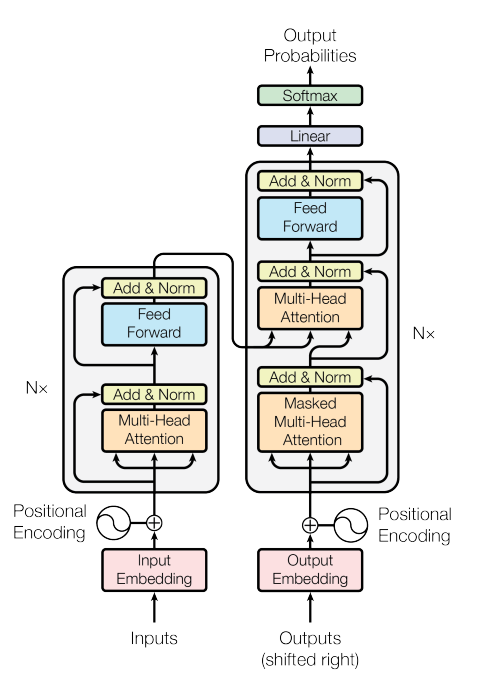
\includegraphics[width=0.8\linewidth]{capitulos/figuras/transformerarquitetura.png}
   \caption{Arquitetura apresenta por \textcite{https://doi.org/10.48550/arxiv.1706.03762}}
   \label{fig:arquitetura}
\end{figure}

A arquitetura do Transformer, baseada na estrutura de codificador-decodificador, desempenha um papel crucial no processamento eficiente de dados. O componente codificador transforma uma sequência de entrada em uma representação interna contínua, enquanto o decodificador utiliza essa representação para gerar a saída desejada de forma sequencial, com cada etapa autorregressiva usando as saídas anteriores como entrada adicional. Essa estrutura é complementada pelo mecanismo de autoatenção, que permite ao modelo capturar dependências de longo alcance de maneira eficaz. Diferentemente das redes neurais convolucionais (CNNs), que capturam características espaciais, ou das redes neurais recorrentes (RNNs), eficazes para dados sequenciais, os Transformers eliminam a necessidade dessas estruturas específicas, utilizando apenas camadas de atenção para lidar com a sequencialidade dos dados. Isso permite uma paralelização mais eficiente durante o treinamento e melhora a capacidade de modelar dependências de longo alcance \cite{THIRUNAVUKARASU2024100648}. 

A arquitetura do codificador-decodificador forma a base da transdução de sequência neuronal \cite{Vaswani2017}. O componente codificador do design converte uma sequência de representações de símbolos de entrada \(x_1, x_2, \ldots, x_n\) em uma sequência contínua \(z_1, z_2, \ldots, z_n\). O componente decodificador produz uma sequência de saída \(y_1, y_2, \ldots, y_m\), um de cada vez. Cada etapa autorregressiva usa os símbolos criados anteriormente como entrada adicional para criar a próxima. Existe uma estrutura de codificador/decodificador com auto-atenção em camadas e camadas ligadas pontualmente dentro do Transformer. A Figura \ref{fig:transformers} ilustra a arquitetura do Transformer mostrando o componente codificador que transforma a sequência de entrada em uma representação interna contínua, e o componente decodificador que gera a sequência de saída de forma sequencial.

\begin{figure}
    \centering
    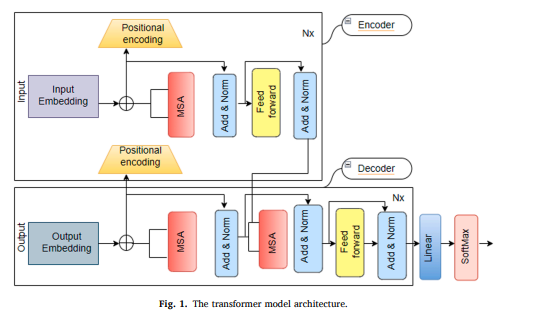
\includegraphics[width=1.0\linewidth]{capitulos//figuras/image_transformer.png}
    \caption{A arquitetura do Transformer codificados de \textcite{THIRUNAVUKARASU2024100648}}
    \label{fig:transformers}
\end{figure}


\textcite{LIN2022111} define a autoatenção como elemento central nas redes Transformers, tendo como objetivo eliminar a necessidade de estruturas recorrentes ou convolucionais, tradicionalmente empregadas para capturar relações temporais ou espaciais em dados sequenciais. A autoatenção confere aos modelos de rede Transformer a capacidade de atribuir diferentes níveis de importância às várias partes de uma sequência de entrada. Isso significa que, ao processar qualquer segmento da sequência, a rede pode efetivamente ponderar a importância em outros segmentos relevantes, identificando e realçando as conexões críticas entre eles. Esse processo não só enriquece a representação do contexto, mas também aprimora a capacidade da rede de interpretar e reagir a padrões complexos nos dados, tornando as redes Transformers extremamente eficazes em aplicações de processamento de linguagem natural e outras tarefas que exigem compreensão de sequências.

No contexto das redes Transformer, a autoatenção é um mecanismo essencial e pode ser descrito matematicamente através de três componentes principais: consultas (\(Q\)), chaves (\(K\)) e valores (\(V\)). Esses componentes são projetados a partir da entrada usando matrizes de pesos aprendidas. A autoatenção é calculada pela seguinte Equação \ref{eq:Attention}.

\begin{equation}
\text{Attention}(Q, K, V) = \text{softmax}\left(\frac{QK^T}{\sqrt{d_k}}\right)V
\label{eq:Attention}
\end{equation}

A Figura \ref{fig:etrans} ilustra o mecanismo de "scaled dot-product attention", onde as consultas (\(Q\)), chaves (\(K\)) e valores (\(V\)) são combinados para calcular a atenção de maneira escalonada, utilizando a divisão por \(\sqrt{d_k}\) para evitar valores extremamente grandes na função softmax, o que poderia levar a gradientes muito pequenos durante o treinamento.

\begin{figure}
    \centering
    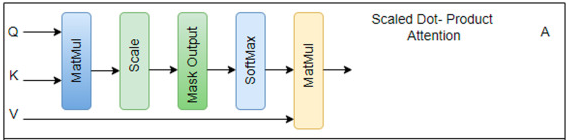
\includegraphics[width=1.0\linewidth]{capitulos//figuras/scalled.png}
    \caption{Mecanismo de atenção por produto escalar escalado (scaled dot-product attention), onde a função de atenção é aplicada utilizando consultas, chaves e valores escalonados.Figura de de \textcite{THIRUNAVUKARASU2024100648}}
    \label{fig:etrans}
\end{figure}

Em contraste com a aplicação de uma única função de atenção, as redes Transformer implementam a estratégia de atenção multi-cabeça. Neste mecanismo, as consultas, chaves e valores originais, que estão em uma dimensão \(d\), são projetados em novas dimensões \(d_q\), \(d_k\) e \(d_v\), respectivamente, usando \(h\) diferentes conjuntos de projeções aprendidas. Para cada um desses conjuntos, a saída é calculada utilizando a função de atenção. O modelo então concatena as saídas de cada uma das cabeças de atenção e as projeta de volta para uma representação unificada de dimensão \(d\), definido pela Equação \ref{eq:MultAttention}.

\begin{equation}
\begin{aligned}
\text{MultiHeadAttn}(Q, K, V) &= \text{Concat}(\text{head}_1, \ldots, \text{head}_h)W^O \\
\text{onde } \text{head}_i &= \text{Attention}(QW_i^{Q}, KW_i^{K}, VW_i^{V})
\label{eq:MultAttention}
\end{aligned}
\end{equation}

A Figura \ref{fig:enter-label} ilustra o mecanismo de "multi-head attention", mostrando como múltiplas cabeças de atenção operam em paralelo, permitindo que o modelo considere diferentes partes da entrada de diferentes maneiras, antes de combinar os resultados.

Na arquitetura do Transformer, existem três tipos de atenção:

1. Autoatenção: Utilizada no codificador Transformer, onde \(Q = K = V\), com \(Q\) representando as saídas da camada anterior.
   
2. Autoatenção mascarada: No decodificador Transformer, a autoatenção é limitada para que as consultas em cada posição só possam atender a posições até aquela específica. Isso é feito aplicando uma máscara à matriz de atenção não normalizada \(QK^T\).

3. Atenção cruzada: As consultas são projetadas a partir das saídas da última camada do decodificador, enquanto chaves e valores são projetados usando as saídas do codificador.

\begin{figure}
    \centering
    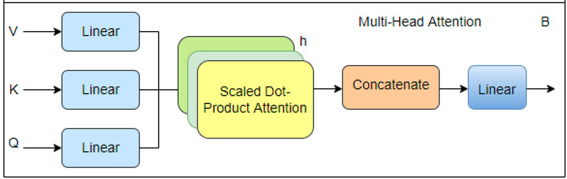
\includegraphics[width=1.0\linewidth]{capitulos//figuras/multi-head.png}
    \caption{Mecanismo de atenção multi-cabeça (multi-head attention), que permite que várias cabeças de atenção operem em paralelo, combinando suas saídas para uma representação final.Figura de de \textcite{THIRUNAVUKARASU2024100648}}
    \label{fig:enter-label}
\end{figure}

Entendendo o conceito geral das redes tranformers vamos apresentar o funcionamento de suas variantes como o Bert de \textcite{Develin}, Roberta de \textcite{Roberta}, Destilbert de \textcite{https://doi.org/10.48550/arxiv.1910.01108}, a Figura ~\ref{fig:linhatransformer} mostra a linha do tempo das arquiteturas transfomers.

\begin{figure}[H]
   \centering
   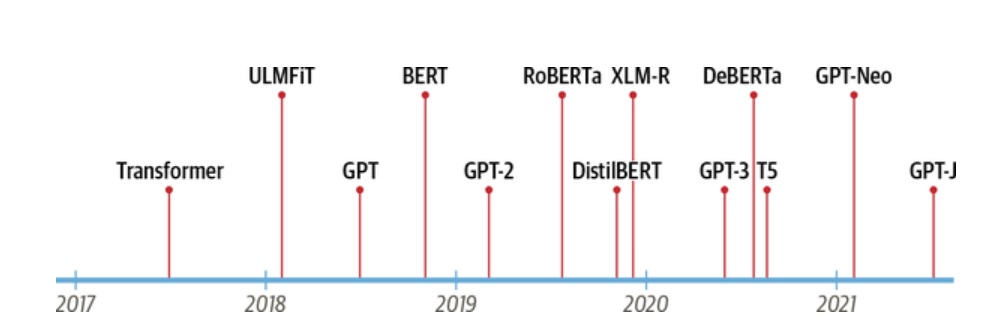
\includegraphics[width=0.8\linewidth]{capitulos/figuras/transformadoras.jpg}
   \caption{Linha do tempo apresentado por  \textcite{Tunstall2022-uq}}
   \label{fig:linhatransformer}
\end{figure}


O BERT (\textit{Bidirectional Encoder Representations from Transformers}) é um modelo de representação de linguagem baseado na arquitetura Transformer. No caso do BERT, durante o pré-treinamento, o modelo é exposto a grandes quantidades de texto não rotulado. Uma das técnicas utilizadas no pré-treinamento do BERT é o masked language modeling (MLM), onde palavras são aleatoriamente ocultadas em uma sequência de entrada e o modelo é treinado para prever as palavras ocultas com base no contexto das palavras circundantes. Isso permite ao BERT capturar o contexto bidirecional de cada palavra em uma frase, pois o modelo não apenas recebe informações de palavras anteriores, mas também de palavras subsequentes. O MLM é implementado aplicando uma máscara a algumas palavras de entrada e treinando o modelo para reconstruir essas palavras com base no contexto global da frase. Essa tarefa de reconstrução força o BERT a aprender representações ricas que capturam o significado das palavras e sua relação com o contexto \cite{Develin}.

Além do MLM, o BERT também emprega a técnica de Next sentence prediction (NSP) durante o pré-treinamento. A NSP envolve a tarefa de prever se uma frase é a próxima em um documento. Essa tarefa auxilia o modelo a capturar o contexto mais amplo de uma sequência de entrada, permitindo que ele entenda como as frases se relacionam umas com as outras. Dessa forma, o BERT aprende a capturar informações de contexto tanto em nível de palavra quanto em nível de frase, o que é crucial para muitas tarefas de processamento de linguagem natural.

Após o pré-treinamento, o BERT pode ser ajustado (fine-tuned) para tarefas específicas de linguagem natural, como classificação de texto, marcação de sequência e resposta a perguntas. Durante o ajuste fino, o modelo é treinado em um conjunto de dados rotulados relacionados à tarefa em questão. Os parâmetros do BERT são atualizados durante o treinamento, permitindo que o modelo se adapte à tarefa específica. Como o BERT já aprendeu representações ricas de linguagem durante o pré-treinamento, ele pode ser ajustado rapidamente para tarefas específicas, aproveitando o conhecimento prévio que adquiriu. Esse ajuste fino é essencial para adaptar o BERT a um domínio específico ou a uma tarefa específica, melhorando seu desempenho e capacidade de generalização.

O BERT se destaca por sua arquitetura unificada, que é aplicada de forma consistente em diferentes tarefas. Sua arquitetura é baseada em um codificador Transformer bidirecional com várias camadas, seguindo a implementação original proposta por \textcite{https://doi.org/10.48550/arxiv.1706.03762} e disponibilizada na biblioteca tensor2tensor. 

É importante ressaltar que, ao contrário do Transformer utilizado no GPT, o Transformer do BERT utiliza autoatenção bidirecional, permitindo que cada token considere o contexto tanto à sua esquerda quanto à sua direita \cite{Develin}. 


% 13 trabalho

No conjunto de estudos revisados, destaca-se o trabalho de \textcite{Reynald}, que utiliza redes transformers na abordagem UViT para estimar a fração de ejeção ventricular esquerda (FEVE) em fluxos de vídeo de ecocardiograma. O modelo UVT (Ultrasound Video Transformer) opera em duas etapas: primeiro, uma rede neural convolucional (ResNetAE) extrai características dos quadros de vídeo de ecocardiografia. Em seguida, um transformador inspirado na arquitetura BERT processa essas características para prever a FEVE, capturando relações temporais entre os quadros. A UViT apresentou um MAE (Erro Médio Absoluto) de 5,95 e R² de 0,52 no conjunto de dados EchoNet-Dynamic, superando o desempenho de outros métodos de aprendizado profundo.

A arquitetura UViT proposta inclui três módulos: um codificador para reduzir a dimensionalidade dos dados, um módulo BERT para raciocínio espaço-temporal, e dois regressores para prever os índices dos quadros de fim de sístole (ES) e fim de diástole (ED), além da FEVE. Na redução da dimensionalidade, um ResNetAE destila os quadros de ultrassom em vetores de 1024 dimensões, que são empilhados formando a incorporação inicial do vídeo (Lote x Quadros x 1024). Esta incorporação é então processada pelo modelo transformer, treinado de ponta a ponta, otimizando o desempenho em tarefas de interpretação de ultrassom cardíaco.

Para capturar relações espaciais-temporais, um encoder BERT é utilizado com uma rede de regressão, formando um modelo de Reconhecimento de Entidades Nomeadas (NER). As incorporações extraídas do ResNetAE são usadas como entrada para o encoder BERT, que contém blocos de autoatenção e atenção, regularizados por camadas de dropout. Após a extração das informações espaciais-temporais pelos encoders BERT e ResNetAE, as características combinadas formam um vetor final, utilizado por dois regressores. O primeiro prevê os índices dos quadros de fim de sístole (ES) e fim de diástole (ED), enquanto o segundo estima a FEVE. Durante o treinamento do regressor da FEVE, são utilizadas perdas combinadas e técnicas de regularização para lidar com o desequilíbrio na distribuição dos valores de FEVE no conjunto de treinamento. A Figura ~\ref{fig:reynaldarq} apresenta uma visão geral da arquitetura proposta para a predição da FEVE em vídeos de ultrassom cardíaco. A operação @ representa o produto escalar entre vetores. Essa arquitetura integrada permite a combinação das informações extraídas de diferentes etapas para uma melhor predição da FEVE em vídeos de ultrassom cardíaco.

\begin{figure}[!ht]
   \centering
   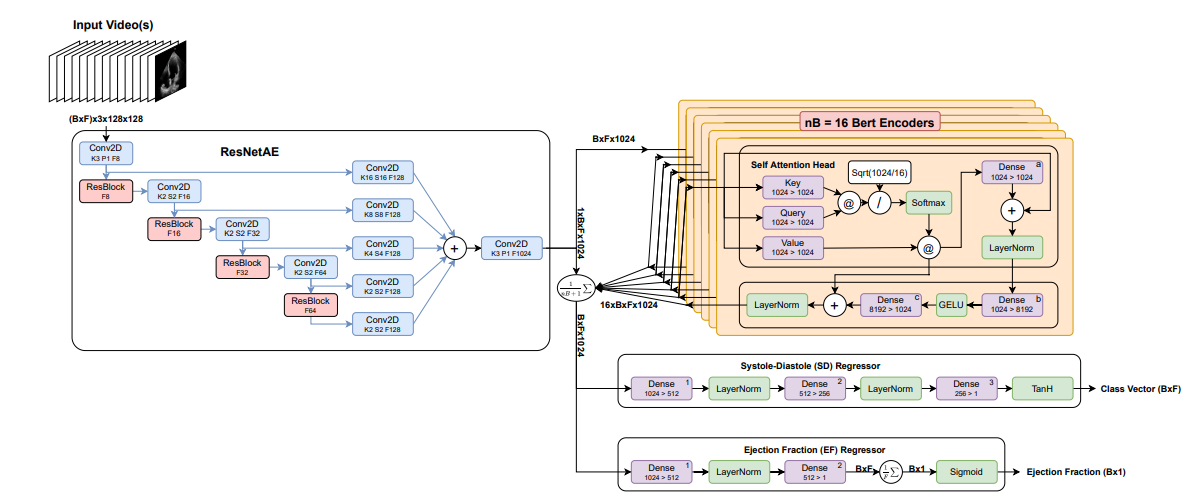
\includegraphics[width=1.0\linewidth]{capitulos/figuras/reynald.png}
   \caption{A Figura apresenta uma visão geral da arquitetura proposta por \textcite{Reynald}.}
   \label{fig:reynaldarq}
\end{figure}

\section{Análise de trabalhos potenciais}
\label{Avaliação de trabalhos potenciais}

Durante a fase inicial de nossa investigação, conduzimos uma revisão sistemática da literatura sobre os métodos predominantes empregados na análise de ecocardiogramas utilizando técnicas de inteligência artificial. Observou-se que a maioria dos estudos recentes recorre predominantemente a redes neurais convolucionais (CNNs). A aplicação  dessas redes foi consistentemente destacada em nossa revisão sistemática da literatura. No entanto, notamos que as melhorias proporcionadas por essas técnicas podem estar se aproximando de um platô em termos de inovação. Esta tendência demonstra a necessidade de explorar novas abordagens tecnológicas para avançar além dos limites atuais.

Especificamente, estudos exemplares como os realizados por \textcite{LIU2021101873}, \textcite{9648607}, e \textcite{9335592}, que utilizam CNNs na análise de ecocardiogramas, com foco em segmentação de imagem e detecção de características cardíacas, confirmam essa observação. Embora esses estudos tenham conseguido avanços significativos, a repetição de abordagens similares e a dependência de incrementos finos na precisão e eficiência podem indicar uma certa maturidade da tecnologia que limita saltos de inovação. Este cenário reflete as conclusões de nossa revisão sistemática, destacando a necessidade de abordagens novas para impulsionar o campo da análise de ecocardiogramas por inteligencia artificial.

A revisão sistemática da literatura revelou que, apesar do vasto número de aplicações, há uma lacuna notável no aproveitamento de tecnologias emergentes como as redes Transformers, que oferecem novas perspectivas para o processamento de dados médicos de imagem. A arquitetura UViT, desenvolvida por \textcite{Reynald}, por exemplo, se destacou pela integração de elementos dos modelos Transformer para analisar sequências de imagens temporais — uma abordagem ainda pouco explorada em ecocardiogramas.

\textcite{Atabansi2023} sugere que os avanços arquiteturais recentes em redes Transformer poderiam oferecer uma nova direção para superar os limites observados com as CNNs, possibilitando uma captura mais eficaz de dinâmicas espaço-temporais complexas, que são cruciais em diagnósticos médicos. Diante deste contexto, propomos adotar e evoluir a arquitetura UViT para analisar ecocardiogramas em nosso trabalho, justificada pela habilidade superior das redes transformadoras de processar sequências de dados complexas. As redes convencionais, embora eficazes em muitas aplicações médicas, apresentam limitações na análise de sequências temporais e na compreensão de contextos mais amplos nas imagens. A arquitetura UViT, que integra elementos de redes Transformer, é particularmente promissora para superar essas limitações. Sua estrutura é desenhada para processar dados não só em um contexto espacial — como é típico nas CNNs — mas também em um contexto temporal, fazendo uso eficiente da autoatenção para entender a relação entre frames sequenciais de um ecocardiograma. Essa capacidade de perceber e integrar informações ao longo do tempo permite uma representação mais rica e detalhada do coração em movimento, potencializando a precisão diagnóstica.

A lacuna atual na aplicação da arquitetura UViT em ecocardiogramas oferece uma oportunidade significativa de inovação. Planejamos implementar e aprimorar a UViT em nossa pesquisa, integrando avanços recentes em técnicas de autoatenção, como RoBERTa e DistilBERT. Essa integração visa refinar a capacidade da rede de processar informações complexas e volumosas, com um foco especial em melhorar a precisão na previsão da fração de ejeção do coração. Além disso, pretendemos expandir a aplicação da UViT para incluir dados de pacientes adultos e pediátricos. Uma explicação  desta estratégia  será apresentada no Capítulo \ref{Metodologia}. 



\pagestyle{ruledheader} %inclui novo capítulo
\chapter{Procedimento Metodológico}
\label{Metodologia}

Este Capítulo detalha o processo metodológico para aprimorar a análise de ecocardiogramas, com foco na melhoria da precisão e eficiência das técnicas de análise de imagens médicas para calcular a fração de ejeção cardíaca. Iniciamos com a revisão sistemática da literatura na Seção \ref{Revisão Sistemática da Literatura} e a avaliação de trabalhos relevantes na Seção \ref{Avaliação de trabalhos potenciais}. Neste Capítulo, a Seção \ref{subsec:descricao_experimentos} descreve os experimentos realizados, enquanto a Seção \ref{Base de dados} aborda a seleção, aquisição e preparação dos conjuntos de dados essenciais. Na Seção \ref{Implementação da arquitetura modificada}, explicamos a implementação de uma arquitetura modificada, seguida pela nova combinação de parâmetros da rede neural na Seção \ref{Otimização de parâmetros}. Por fim, a Seção \ref{sub:Implementação} apresenta as tecnologias utilizadas na execução dos experimentos. A Figura \ref{fig:procedimento_metodologico} ilustra o fluxograma do processo metodológico adotado, abrangendo desde a revisão da literatura até a modificação dos parâmetros da rede neural.

\begin{figure}
    \centering
    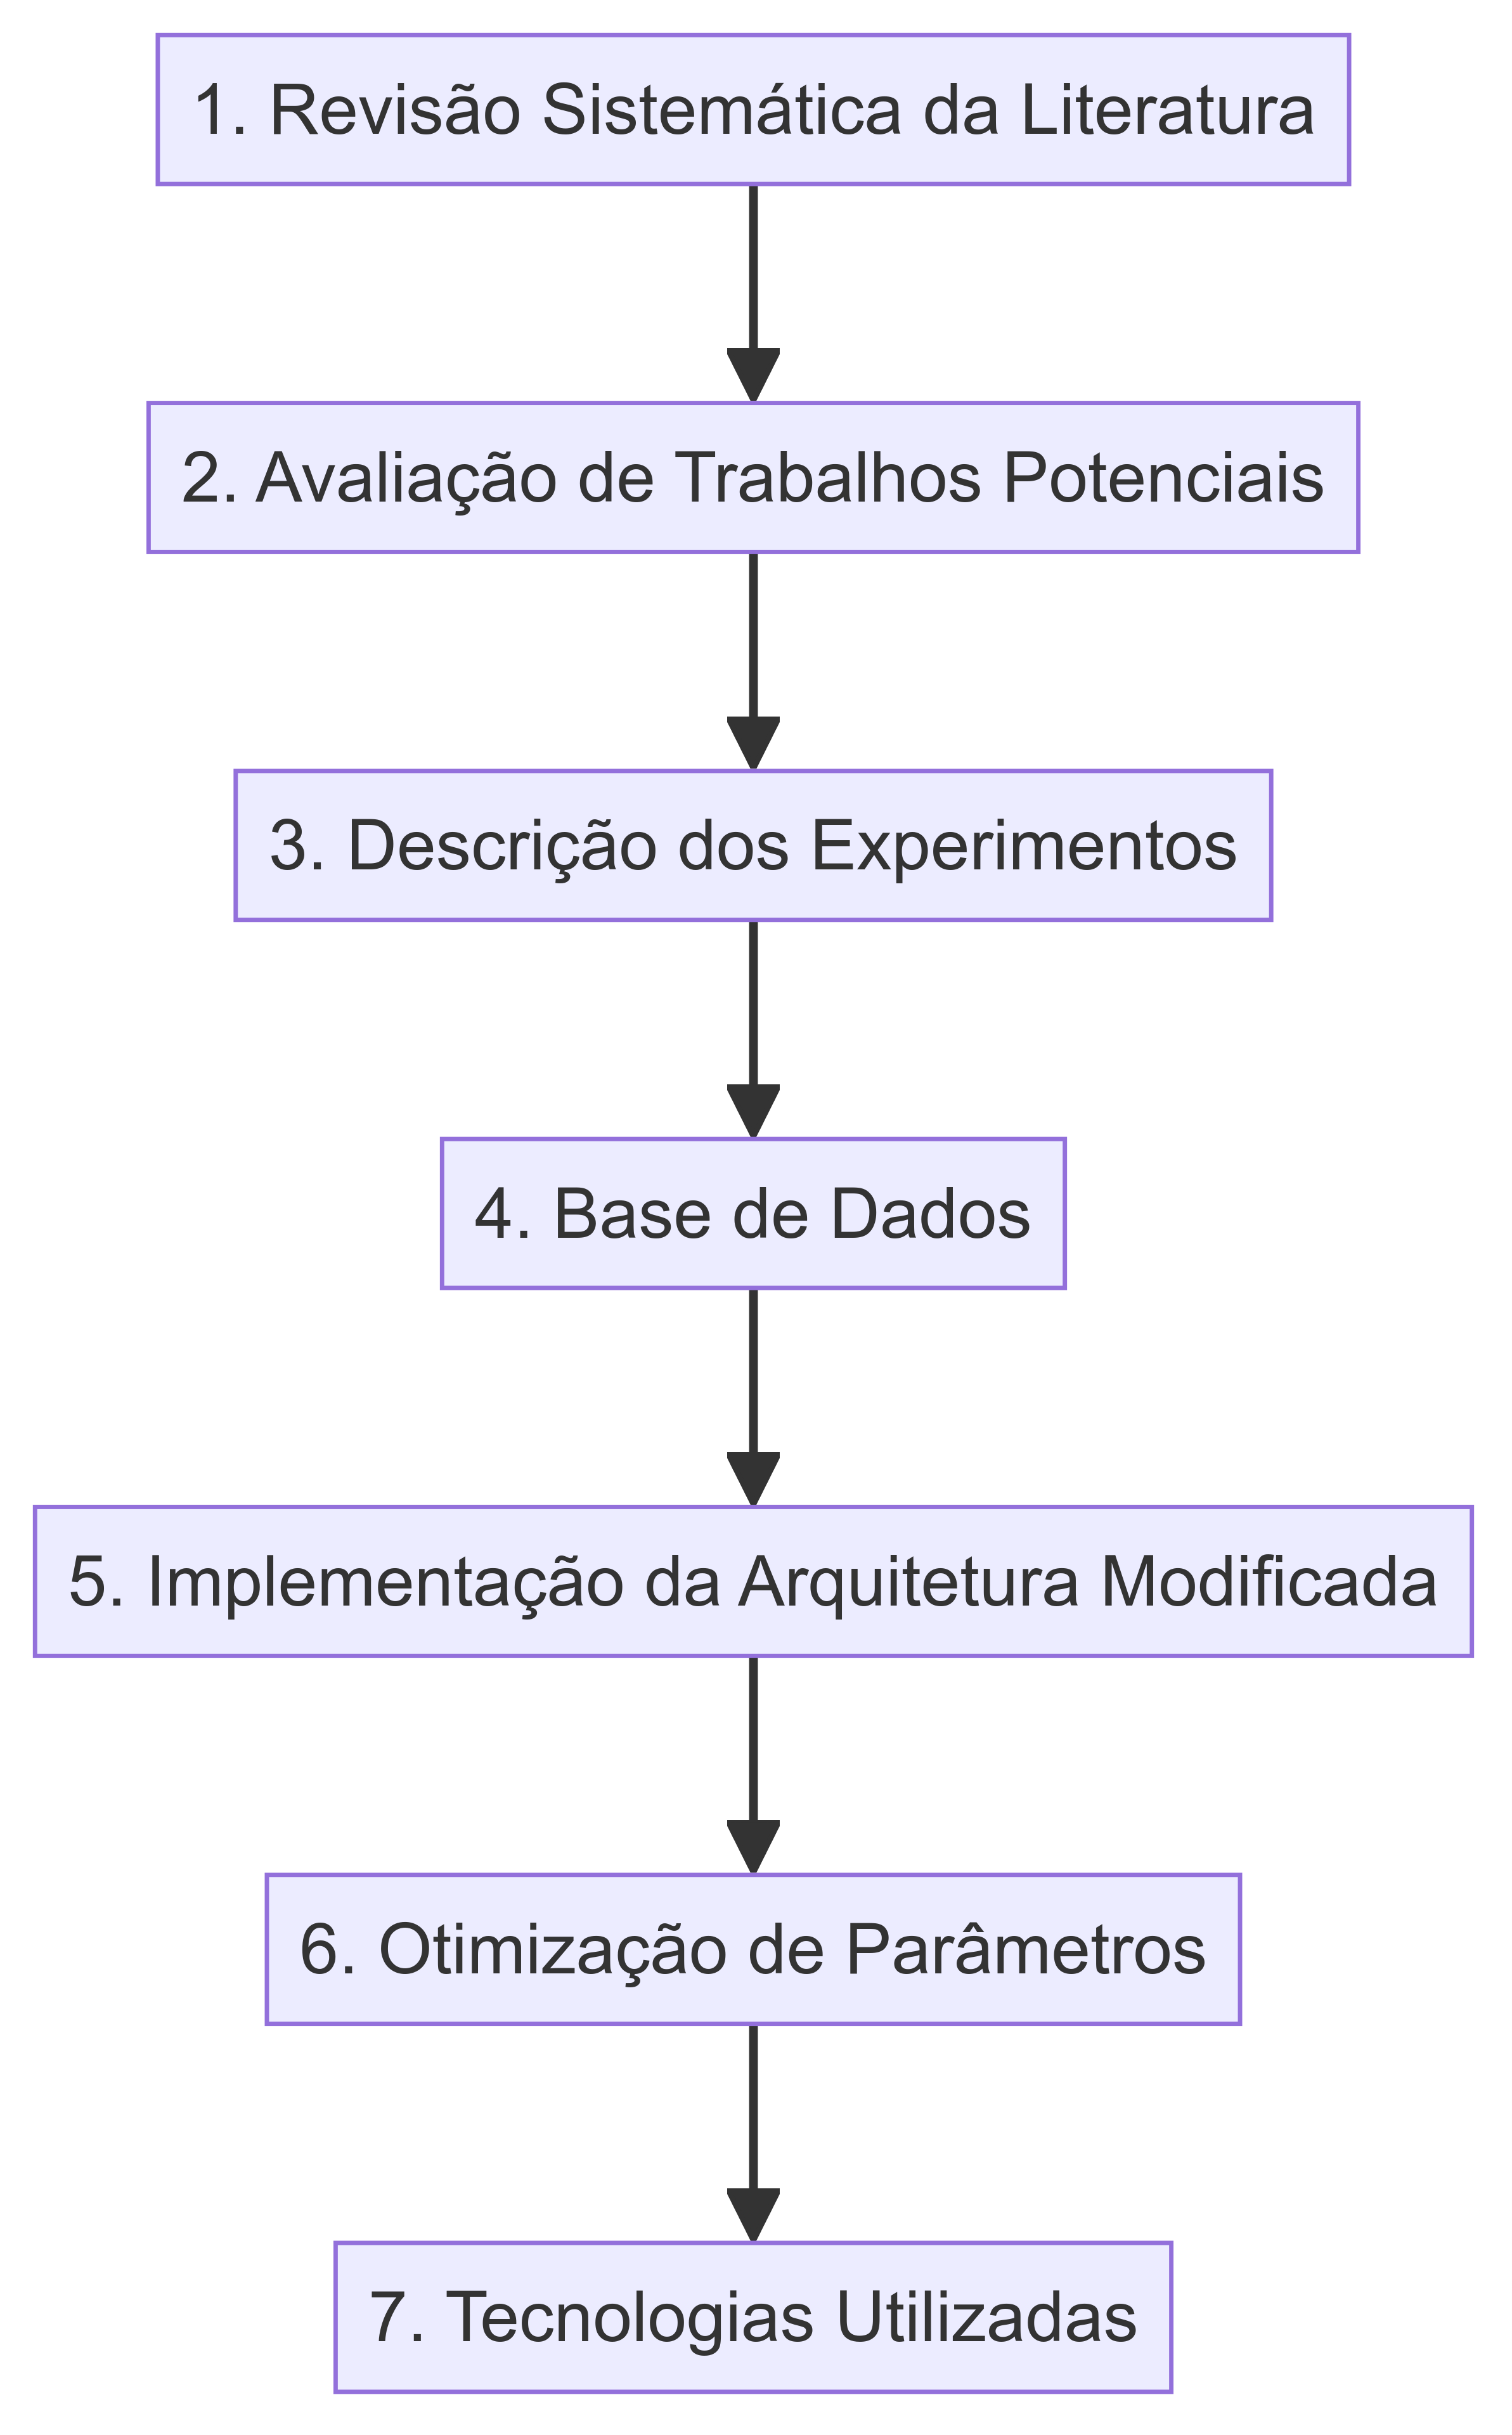
\includegraphics[width=0.5\linewidth]{capitulos//figuras/procedimentometo.png}
    \caption{Fluxograma do processo metodológico para análise de ecocardiogramas visando a melhoria da precisão e eficiência na determinação da fração de ejeção cardíaca.}
    \label{fig:procedimento_metodologico}
\end{figure}


\section{Descrição dos experimentos e justificativa}
\label{subsec:descricao_experimentos}

Foram realizados dois experimentos para avaliar a eficácia da arquitetura UViT e suas adaptações com diferentes bases de dados. O primeiro experimento utilizou a arquitetura UViT exatamente como desenvolvida por \textcite{Reynald} e descrita na Seção \ref{subsec:Redes neurais transformers}, juntamente com os conjuntos de dados do Echonet descritos na Seção \ref{Base de dados}. Este passo inicial é fundamental para estabelecer um ponto de referência comparativo (baseline), permitindo-nos avaliar posteriormente as vantagens e aprimoramentos introduzidos pelas metodologias subsequentes. Em seguida, avançamos para um segundo experimento, que envolve a versão adaptada da arquitetura UViT, que sera detalhada na Seção  \ref{Implementação da arquitetura modificada} e e nova combinação de parâmetros da rede neural na Seção \ref{Otimização de parâmetros}. Esta adaptação foi  aplicada aos conjuntos de dados Echonet e Echoped treinados de formas separadas e um experimento treinado de forma conjunta a fim de validar a hipótese de generalização dos dados. A comparação direta entre a arquitetura UViT clássica e sua versão modificada permite não apenas avaliar o impacto das alterações propostas, mas também destacar as melhorias específicas para dados pediátricos.

A escolha desses dois experimentos foi estratégica para permitir uma análise comparativa efetiva, fundamentando a importância das modificações na arquitetura UViT frente ao método original. A inclusão de dados pediátricos e a comparação dos resultados obtidos fornecem uma base para validar as vantagens das inovações implementadas, oferecendo uma contribuição significativa à precisão da estimativa da fração de ejeção em um contexto ampliado.

\section{Base de dados}
\label{Base de dados}

A escolha das bases de dados \textit{EchoNet-Dynamic} disponibilizado por \cite{Ouyang2020} e \textit{EchoNet Pediátricos} disponibilizado por \cite{Reddy2023} evidencia a intenção de incluir tanto a população adulta quanto a pediátrica, o que resulta em uma significativa extensão do alcance potencial da arquitetura UViT modificada.

A base de dados da  EchoNet-Dynamic contém 10.030 vídeos de ecocardiogramas apicais de 4 câmaras, coletados entre 2016 e 2018 no Hospital da Universidade de Stanford. Cada vídeo disponibilizado foi preparado, removendo textos e informações irrelevantes e padronizado para um formato de 112x112 pixels. Esta padronização é crucial para garantir a consistência e a qualidade dos dados para análises computacionais. Além dos vídeos, a EchoNet-Dynamic oferece medições clínicas e cálculos realizados por sonografistas registrados e verificados por um ecocardiografista de nível 3. Um dos principais indicadores clínicos presentes na base de dados é a fração de ejeção do ventrículo esquerdo, um parâmetro chave para o diagnóstico de cardiomiopatias, avaliação da elegibilidade para certas quimioterapias e determinação da necessidade de dispositivos médicos. Esta métrica é expressa como uma porcentagem, calculada pela razão do volume sistólico final  e o volume diastólico final do ventrículo esquerdo. A base de dados  também inclui traçados do ventrículo esquerdo, realizados no limite endocardíaco em dois momentos distintos: no final da sístole e no final da diástole. Estes traçados são utilizados para estimar o volume ventricular, integrando a área do ventrículo ao longo do eixo maior. Os traçados dos especialistas são representados por um conjunto de coordenadas emparelhadas, correspondentes a cada traçado humano. Estas coordenadas ajudam a determinar a orientação e o tamanho dos eixos do ventrículo esquerdo. A base de dados se encontra disponível em https://echonet.github.io/dynamic/. Acesso em: 03, Agosto de 2023.

A Echoped foi desenvolvido focando exclusivamente em dados pediátricos. Este conjunto de dados compreende 7.643 vídeos de ecocardiografia, cobrindo uma ampla gama de condições típicas de aquisição de imagens em laboratórios de ecocardiografia. Além de incluir medições como a fração de ejeção e volumes do ventrículo esquerdo no final da sístole e diástole. Os vídeos de ecocardiograma do conjunto de dados incluem imagens apicais de 4 câmaras e vistas do eixo curto parasternal, provenientes de pacientes atendidos no Lucile Packard Children’s Hospital em Stanford entre 2014 e 2021. Cada vídeo passou por um processo de edição para garantir a remoção de informações irrelevantes e padronização para o formato de 112x112 pixels, visando a consistência necessária para análises de alta qualidade.As medições clínicas vinculadas a cada vídeo, obtidas e verificadas por especialistas, adicionam um valor inestimável ao conjunto de dados. A métrica da fração de ejeção do ventrículo esquerdo. Além disso, os traçados especializados do ventrículo esquerdo, em momentos específicos do ciclo cardíaco, fornecem dados precisos para estimativas de volume ventricular. A base de dados se encontra disponível em https://echonet.github.io/pediatric/. Acesso em: 28, julho de 2023.


\section{Implementação da arquitetura modificada}
\label{Implementação da arquitetura modificada}

Nessa Seção descrevemos a elaboração e aprimoramento do pipeline para análise de imagens de ecocardiograma, iniciando com a arquitetura base UViT, conforme descrito por \textcite{Reynald}. O primeiro elemento deste pipeline foi projetado para enfrentar os desafios computacionais associados ao processamento de imagens completas de ultrassom, especialmente em formatos de vídeo. Esta etapa foca na manipulação eficiente dos frames de vídeo, que são as imagens individuais sequenciadas para formar o vídeo completo. Adotamos uma estratégia de redução de dimensionalidade, utilizando a Seção de codificação de uma Arquitetura de Autoencoder Residual (ResNetAE), como ilustrado na Figura \ref{fig:resnetAE}. Esta abordagem converte os frames em representações vetoriais compactas, reduzindo significativamente a carga computacional na análise direta das imagens.

A manutenção dessa abordagem específica é crucial, caracterizando-se pela incorporação de blocos residuais em múltiplas escalas tanto no codificador quanto no decodificador. Essa configuração permite uma agregação eficiente de informações através das dimensões espaciais das imagens, facilitando a captura de características relevantes em diferentes níveis de granularidade. Esta estratégia revela-se particularmente vantajosa para a análise complexa de imagens de ultrassom. Além disso, a otimização de hiperparâmetros, que inclui ajustes na profundidade do codificador e no tamanho do espaço latente, é crítica para a configuração da arquitetura do Autoencoder. Este processo de otimização, realizado através de uma tarefa de reconstrução especificamente adaptada ao conjunto de dados de ultrassom, assegura que a arquitetura esteja finalmente sintonizada com as características únicas desses dados, maximizando assim o desempenho e a precisão do modelo.

Prosseguindo nesta direção, a configuração ótima do codificador, resultante deste processo de otimização, é reintegrada ao pipeline como o componente essencial de codificação. Assim, cada quadro é processado pelo codificador transformando-se em um vetor de 1024 dimensões. As representações vetoriais resultantes são organizadas para formar a representação vetorial inicial do clipe, estruturado em uma matriz Batch (lote de dados, representando a quantidade de exemplos de treinamento processados em conjunto) × Nframes (número de quadros, indicando a quantidade de imagens ou frames de vídeo no clipe) × 1024. Esta etapa, importante para a preparação dos dados para análise subsequente, mantém-se inalterada em relação à estratégia original, preservando a abordagem estabelecida para a redução de dimensionalidade.


\begin{figure}
    \centering
    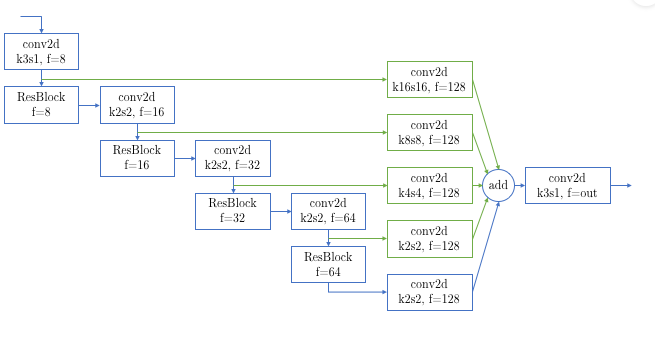
\includegraphics[width=1\linewidth]{image.png}
   \caption{Arquitetura ResNetAE de \textcite{ResNetAE} }
    \label{fig:resnetAE}
\end{figure}

No desenvolvimento do segundo módulo da arquitetura Ultrassom Video Transformer (UViT), houve uma significativa incorporação de tecnologias provenientes do processamento de linguagem natural (PLN), mais notavelmente RoBERTa (Robustly optimized BERT approach). Estes avanços metodológicos são fundamentais para a análise de conteúdo visual e são particularmente eficazes no tratamento de vídeos de ultrassom, promovendo uma compreensão espaço-temporal aprimorada.

RoBERTa, que evolui a partir do BERT (Bidirectional Encoder Representations from Transformers), se sobressai por sua extensiva capacidade de treinamento em vastos conjuntos de dados e um número incrementado de iterações, o que resulta em uma análise mais detalhada dos aspectos espaço-temporais dos vídeos. Uma mudança crítica na transição do BERT para o RoBERTa é a remoção do objetivo de Previsão de Próxima Sentença (NSP), o que foi demonstrado por \textcite{Roberta} manter ou até mesmo aprimorar o desempenho em diversas tarefas de PLN. O RoBERTa também se beneficia do uso de lotes de dados maiores e sequências mais extensas durante o treinamento, o que diverge do protocolo original do BERT e contribui para um avanço na modelagem de linguagem mascarada e na precisão de tarefas específicas de linguagem natural.

A escolha de RoBERTa para a arquitetura UViT permite uma análise mais profunda e detalhada, maximizando a eficácia na interpretação de vídeos de ecocardiograma. Tal mudança não apenas eleva o padrão de análise espaço-temporal para vídeos de ultrassom, mas também estabelece um novo paradigma para a aplicação de técnicas de PLN na análise visual, evidenciando o potencial transformador de adaptar e combinar metodologias de inteligência artificial novas como as redes transformers.

Para conduzir análises espaço-temporais em vídeos de durações variáveis, utilizamos um modelo de Reconhecimento de Entidades Nomeadas (\textit{NER}) baseado em vídeo. Este modelo emprega incorporações vetoriais derivadas de uma etapa de codificação com o uso de ResNetAE (\textit{Autoencoder Residual}) de \textcite{ResNetAE}, que codifica as características visuais essenciais do vídeo. As incorporações vetoriais resultantes são fundamentais e são processadas pelos codificadores RoBERTa. A função de cada codificador, indexada por \(k\), é matematicamente representada pela Equação \ref{eq:encoder_function}.

\begin{equation}
B_k(E) = \text{LayerNorm}\left(D_{k,c}\left(\text{GELU}\left(D_{k,b}\left(A_k(E)\right)\right)\right) + S_k(E)\right),
\label{eq:encoder_function}
\end{equation}

No contexto das redes Transformer, \(S_k(E)\) denota o bloco de Autoatenção, que é responsável por calcular os pesos de atenção normalizados. Esses pesos são derivados do produto escalar entre as matrizes de Consulta (\(Q_k(E)\)) e Chave (\(K_k(E)\)), ajustados por um fator de escala. Este fator é dependente da relação entre a dimensionalidade das incorporações vetoriais (\(n_d\)) e o número de cabeças de atenção (\(n_B\)). A equação correspondente é apresentada em \ref{eq:self_attention}. Uma explicação mais detalhada sobre redes Transformer e seus componentes é fornecida na Seção \ref{subsec:Redes neurais transformers}.



\begin{equation}
S_k(E) = \text{Softmax}\left(\frac{Q_k(E)K_k^T(E)}{\sqrt{\frac{n_d}{n_B}}}\right)V_k(E),
\label{eq:self_attention}
\end{equation}


E \(A_k(E)\) indica o bloco de Atenção, integrando as saídas de \(S_k(E)\) com as incorporações vetoriais originais \(E\), seguido por uma camada de normalização, também conhecida como Layer Normalization, é uma etapa crítica no processamento dos incorporações vetoriais e é dada pela Equação \ref{eq:attention_integration}.

\begin{equation}
A_k(E) = \text{LayerNorm}\left(D_{k,a}\left(S_k(E)\right) + E\right).
\label{eq:attention_integration}
\end{equation}

Neste cenário avançado, as matrizes \( Q _k \), \( K_k \), e \( V_k \) atuam como transformações lineares essenciais, designadas respectivamente às funções de Consulta (Query), Chave (Key) e Valor (Value), fundamentais na arquitetura de autoatenção. Estas matrizes são responsáveis por converter os dados de entrada em representações mais significativas que facilitam a identificação de padrões relevantes para a tarefa em questão. As camadas \( D_{k,\{a,b,c\}} \)  representam camadas densas intermediárias que exercem uma função crítica na reformulação dos dados processados pelo codificador, permitindo uma manipulação mais refinada das informações. Os parâmetros ajustáveis \( n_B \) e \( n_D \) referentes ao tamanho do batch e à dimensão dos embeddings, respectivamente, são  calibrados para encontrar um equilíbrio ótimo entre a capacidade de processamento e a eficiência computacional. Este ajuste fino visa aprimorar o desempenho do modelo na análise de vídeos de ecocardiograma, garantindo que o sistema seja capaz de processar informações complexas de forma eficaz, sem comprometer a rapidez e a precisão das previsões. A otimização desses parâmetros é um processo iterativo que envolve a experimentação e a validação cruzada para assegurar que o modelo esteja ajustado para oferecer a melhor performance possível.

No terceiro componente do nosso pipeline de análise de vídeos, a integração das saídas dos $k$ codificadores, seja eles para o RoBERTa do módulo anterior, denotadas por $B_k(E)$, com a saída do ResNetAE, $E$, é realizada por meio de uma média ponderada. Esta abordagem visa combinar  as representações espaço-temporais capturadas pelos codificadores RoBERTa com as características espaciais codificadas pelo ResNetAE. A formulação matemática para a matriz de características composta $M(E)$ é dada pela Equação \ref{eq:equacao_norm}.


\begin{equation}
M(E) = \frac{1}{n_B + 1} \left( E + \sum_{k=1}^{n_B} B_k(E) \right),
\label{eq:equacao_norm}
\end{equation}

onde:
\begin{itemize}
    \item $E$ representa as incorporações vetoriais obtidas pela aplicação do ResNetAE sobre as imagens de ultrassom, funcionando como a base para características espaciais.
    \item $B_k(E)$ é a matriz de saída do $k$-ésimo codificador, seja RoBERTa, que foi aplicado para potencializar $E$ com informações espaço-temporais. Esta matriz contém vetores de embedding para cada elemento processado, com cada vetor representando a informação espaço-temporal enriquecida de um único frame ou segmento de vídeo. A dimensão da matriz reflete o número de elementos processados e a dimensão dos embeddings gerados pelo codificador.
    \item $n_B$ indica o número total de codificadores RoBERTa empregados, possibilitando uma análise detalhada e diversificada através da combinação de múltiplas representações espaço-temporais.
    \item $M(E)$ é a matriz de características composta, que integra as dimensões espaciais e espaço-temporais em uma única representação. Esta matriz é o resultado da combinação ponderada de $E$ com as saídas $B_k(E)$ de todos os codificadores utilizados, fornecendo uma base rica e multifacetada para a fase de regressão subsequente.
\end{itemize}


A eficácia desta abordagem combinatória origina-se da integração de duas dimensões essenciais na análise de imagens de ultrassom. Primeiramente, exploramos a dimensão espacial, que envolve a análise da estrutura e anatomia visíveis nas imagens. Utilizando o ResNetAE, não só reduzimos a dimensionalidade das imagens para facilitar o processamento subsequente, mas também extraímos características físicas, como por exemplo a forma do coração e a textura dos tecidos. Esta análise é fundamental para entender a condição estrutural do órgão. Em seguida, adicionamos a dimensão espaço-temporal, que capta as variações e movimentos ao longo do tempo, essenciais para analisar os ciclos cardíacos. Essa dimensão é reforçada pelos codificadores RoBERTa, que analisam a sequência dos quadros para detectar padrões de movimento, como expansão e contração durante a sístole e diástole.

Essas duas dimensões são então integradas em uma única matriz de características, denominada \(M(E)\). Esta matriz representa um conjunto compacto e integrado de dados que combina informações espaciais e espaço-temporais. O processo envolve a agregação de vetores de características extraídos de cada quadro de vídeo, resultando em uma representação unificada que potencializa a análise e a precisão dos modelos de regressão. A precisão aprimorada obtida com \(M(E)\) é crucial para identificar com exatidão os momentos específicos dos ciclos cardíacos, como os pontos de início e fim da sístole e diástole, além de calcular a fração de ejeção.


Essa matriz \(M(E)\) é submetida a dois regressores: um destinado a prever os índices de início da sístole (ES) e diástole (ED) mostrado na figura \ref{fig:reg01}, \(R_{SD}(M(E))\), e outro para calcular a Fração de Ejeção do Ventrículo Esquerdo mostrado na Figura \ref{fig:fraceject} , \(R_{EF}(M(E))\). O regressor \(R_{SD}\) é formulado como a saída de três camadas lineares intercaladas com normalização por camadas, finalizando com uma ativação tangente hiperbólica (tanh). A função tanh é escolhida por sua eficácia em normalizar a saída do modelo para um intervalo entre -1 e 1, facilitando a estabilização do treinamento e a interpretação dos resultados finais. A fração de ejeção do ventrículo esquerdo é expressa pela Equação \ref{eq:01}, com \(n_F\) representando o número de quadros de entrada. A rede de regressão reduz a dimensão das incorporações vetoriais para 1 para cada quadro de entrada, e a média dessas previsões individuais produz uma única estimativa de fração de ejeção do ventrículo esquerdo por vídeo. Este processo de redução de dimensões é importante, pois transforma dados complexos e de alta dimensionalidade em uma forma mais tratável que enfatiza as características mais relevantes para a tarefa de predição, maximizando a eficiência computacional e a precisão do modelo.


\begin{equation}
R_{EF}(M(E)) = \text{Sigmoid} \left( \frac{1}{n_F} \sum_{f=1}^{n_F} D_{EF,2} \left( \text{LayerNorm} \left( D_{EF,1} (M(E)) \right) \right) \right)
\label{eq:01}
\end{equation}



\begin{figure}
    \centering
    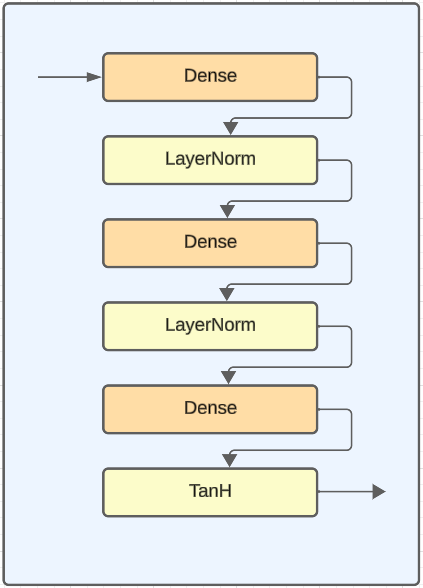
\includegraphics[width=0.5\linewidth]{imagereg.png}
    \caption{Ramo de regressão sistole-diástole}
    \label{fig:reg01}
\end{figure}



\begin{figure}
    \centering
    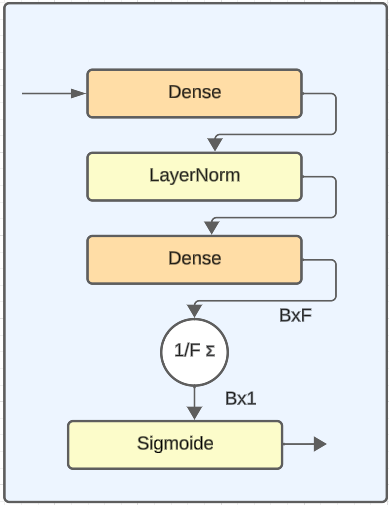
\includegraphics[width=0.5\linewidth]{reg02.png}
    \caption{Ramo de regressão para calculo da fração de ejeção}
    \label{fig:fraceject}
\end{figure}


Para otimizar a precisão na previsão da Fração de Ejeção do Ventrículo Esquerdo, adotamos uma abordagem de treinamento que integra tanto a minimização de erros quanto a aplicação de \textit{regularização}, visando corrigir desequilíbrios na distribuição de fração de ejeção do ventrículo esquerdo no conjunto de dados. As métricas de erro empregadas são o \textit{Mean Squared Error} (\textit{MSE}) e o \textit{Mean Absolute Error} (\textit{MAE}), definidos respectivamente pelas Equações \ref{eq:MSE} e \ref{eq:MAE}.

\begin{equation}
L_{\text{MSE}}(\hat{y}, y) = \frac{1}{n_F} \sum_{f=1}^{n_F} (\hat{y}_f - y_f)^2,
\label{eq:MSE}
\end{equation}

Na Equação \ref{eq:MSE}, \(L_{\text{MSE}}(\hat{y}, y)\) é a função de perda MSE, onde \(\hat{y}\) é o valor previsto, \(y\) é o valor real, e \(n_F\) é o número total de quadros de entrada. A função de perda MSE calcula a média dos quadrados das diferenças entre os valores previstos e reais.

\begin{equation}
L_{\text{MAE}} = \frac{1}{n_F} \sum_{f=1}^{n_F} \left| \hat{y}_f - y_f \right|,
\label{eq:MAE}
\end{equation}

Na Equação \ref{eq:MAE}, \(L_{\text{MAE}}\) é a função de perda MAE, onde \(\hat{y}\) é o valor previsto, \(y\) é o valor real, e \(n_F\) é o número total de quadros de entrada. A função de perda MAE calcula a média das diferenças absolutas entre os valores previstos e reais.


A fim de enfatizar o treinamento na estimativa da fração de ejeção do ventrículo esquerdo e mitigar desvios significativos das previsões em relação a um valor de referência $\gamma$ — aproximadamente a média da fração de ejeção do ventrículo esquerdo no conjunto de treinamento —, introduzimos um termo de regularização $R(y)$, conforme a Equação \ref{eq:Reg}.

\begin{equation}
R(y) = (1 - \alpha) + \alpha \cdot \frac{\lVert y - \gamma \rVert}{\gamma},
\label{eq:Reg}
\end{equation}

O parâmetro $\alpha$ calibra a intensidade da penalidade para estimativas de Fração de Ejeção do Ventrículo Esquerdo (FEVE) que divergem do valor de referência $\gamma$, proporcionando uma sintonia refinada na penalização de desvios do alvo FEVE.

Assim, a função de custo total $L_{EF}$, que o modelo visa minimizar durante o processo de treinamento, é formulada pela combinação das métricas de erro ponderadas pelo termo de regularização, conforme expresso pela Equação \ref{eq:LEF}.


\begin{equation}
L_{EF} = (L_{MSE} + L_{MAE}) \cdot R(y).
\label{eq:LEF}
\end{equation}

Esta formulação assegura que, além de aprender a reduzir os erros de previsão diretamente, o modelo ajusta suas estimativas para alinhar-se mais estreitamente com a distribuição esperada de fração de ejeção do ventrículo esquerdo no conjunto de treinamento, abordando assim os desafios impostos por possíveis desequilíbrios na distribuição das fração de ejeção do ventrículo esquerdo.

\section{Nova combinação de hiperparâmetros}
\label{Otimização de parâmetros}

Essa Seção busca aprimorar o desempenho do novo modelo em comparação ao descrito por \textcite{Reynald}. Uma reconfiguração dos hiperparâmetros foi executada. Assim, ampliamos o \textit{Attention Head} de 16 para 32, o que amplia a capacidade do modelo de processar informações em paralelo, melhorando significativamente a atenção aos detalhes sutis nos dados e reforçando a capacidade de generalização. 

Além disso, o incremento do \textit{Number of Hidden Layers} de 16 para 32 permite ao modelo captar e representar hierarquias mais sofisticadas de características, essenciais para a compreensão aprofundada de contextos e relações complexas nos dados. Essa representação aprimorada é um fator determinante para o aumento da precisão das previsões.

A duplicação do \textit{Batch Size} contribui não apenas para a eficiência computacional, permitindo que o modelo processe mais dados em simultâneo e acelere o treinamento, mas também promove uma estimativa do gradiente mais robusta, ajudando a mitigar o risco de \textit{overfitting}.

Para otimizar a utilização dos recursos de memória da GPU, o \textit{Max Length (dsmax)} foi reduzido de 128 para 64, prevenindo a exaustão da memória e garantindo a eficácia do treinamento. Este ajuste é uma medida preventiva que assegura a operacionalidade do modelo dentro das limitações de hardware, mantendo a qualidade do treinamento apesar do aumento das demandas computacionais devido às camadas adicionais e ao tamanho do lote expandido.
Esta etapa busca aprimorar o desempenho do novo modelo em comparação ao descrito por \textcite{Reynald}. Uma reconfiguração dos hiperparâmetros foi executada. Assim, ampliamos o \textit{Attention Head} de 16 para 32, o que amplia a capacidade do modelo de processar informações em paralelo, melhorando significativamente a atenção aos detalhes sutis nos dados e reforçando a capacidade de generalização.

Além disso, o incremento do \textit{Number of Hidden Layers} de 16 para 32 permite ao modelo captar e representar hierarquias mais sofisticadas de características, essenciais para a compreensão aprofundada de contextos e relações complexas nos dados. Essa representação aprimorada é um fator determinante para o aumento da precisão das previsões.

A duplicação do \textit{Batch Size} contribui não apenas para a eficiência computacional, permitindo que o modelo processe mais dados em simultâneo e acelere o treinamento, mas também promove uma estimativa do gradiente mais robusta, ajudando a mitigar o risco de \textit{overfitting}.

Para otimizar a utilização dos recursos de memória da GPU, o \textit{Max Length (dsmax)} foi reduzido de 128 para 64, prevenindo a exaustão da memória e garantindo a eficácia do treinamento. Este ajuste é uma medida preventiva que assegura a operacionalidade do modelo dentro das limitações de hardware, mantendo a qualidade do treinamento apesar do aumento das demandas computacionais devido às camadas adicionais e ao tamanho do lote expandido.

Os seguintes parâmetros não foram modificados, com as seguintes justificativas: A *taxa de aprendizado (learning rate, lr)* foi mantida em \(1 \times 10^{-5}\) (a velocidade com que o modelo aprende com os dados durante o treinamento). Essa taxa é escolhida para garantir um aprendizado controlado e estável, minimizando oscilações bruscas durante o treinamento que poderiam prejudicar a convergência do modelo. A *dimensão latente (latent\_dim)* continua em 1024 (o tamanho do vetor que representa as características aprendidas dos dados). Identificamos que uma alteração nesse parâmetro não traria benefícios adicionais, uma vez que essa configuração já provou ser suficiente para capturar as características essenciais dos dados, e aumentá-la resultaria em um modelo muito grande, incapaz de ser processado na GPU disponível, sem trazer os benefícios esperados. O *período de passo da taxa de aprendizado (lr\_step\_period)* é mantido em 3 épocas (a frequência com que a taxa de aprendizado é ajustada para garantir eficiência), que é o intervalo antes da taxa de aprendizado ser dividida por 10. Esse procedimento permite uma redução gradual e controlada da taxa, facilitando uma convergência mais estável e eficiente do modelo. Finalmente, o *espaçamento mínimo entre quadros (ds\_min\_spacing)* foi mantido em 10 quadros (o número mínimo de quadros entre amostras durante o treinamento) para assegurar que a densidade dos quadros processados seja adequada, evitando sobrecarga de processamento e garantindo uma boa representação temporal dos dados. Essas decisões visam otimizar o processo de treinamento, mantendo a eficácia e a eficiência do modelo.

Todas essas modificações foram implementadas com a premissa de que um modelo com maior capacidade e eficiência computacional pode aprender representações mais complexas e abstratas dos dados


\section{Implementação} 
\label{sub:Implementação}

Na quinta etapa do projeto, foi estabelecido um ambiente de desenvolvimento utilizando \textit{Docker}, garantindo isolamento e reprodutibilidade nas execuções da implementação e testes. Esse ambiente operou com a linguagem \textit{Python} e utilizou as bibliotecas \href{https://pytorch.org/}{\textit{PyTorch}} e \href{https://huggingface.co/transformers/}{\textit{transformers}}, que são reconhecidas por sua ampla funcionalidade em projetos de aprendizado de máquina e inteligência artificial. A estrutura de processamento paralelo foi implementada utilizando oito placas de GPU \textit{Tesla Pascal} (modelo P100-SXM2-16GB), cada uma equipada com 16GB de memória e 3584 \textit{cores CUDA}, totalizando 28672 \textit{cores CUDA}. Esse \textit{setup} permitiu uma execução paralela eficaz, sendo crucial para o processamento de grandes volumes de dados e análise computacional intensiva.

Para suportar as elevadas demandas de processamento, a máquina escolhida para este ambiente estava equipada com dois processadores \textit{Intel Xeon E5-2698 v4}, cada um com 20 cores e 40 \textit{threads}, somando um total de 40 cores físicas e 80 \textit{threads} lógicas. Além disso, a máquina foi configurada com 512 GB de RAM e um armazenamento em \textit{SSD} de 7TB, proporcionando uma capacidade adequada para a manipulação eficiente de dados e execução de operações que requerem intensa utilização de memória.

O modelo desenvolvido está disponível em \url{https://github.com/thiago092/UVIT_MODIFICADO/}



\pagestyle{ruledheader} %inclui novo capítulo
\chapter{Resultados}
\label{sec:resultados}

A Tabela \ref{tab:comparativo} apresenta uma análise detalhada do desempenho do modelo UViT clássico comparado com suas versões modificadas, aplicadas a conjuntos de dados pediátricos, adultos e combinados. Este comparativo inclui mudanças percentuais nas métricas de desempenho Erro Médio Absoluto (MAE), Erro Quadrático Médio Raiz (RMSE) e Coeficiente de Determinação \( R^2 \), destacando tanto melhorias quanto regressões em relação ao modelo baseline.

\begin{table}[htbp]
\centering
\small % Diminui a fonte da tabela
\caption{Comparativo das variações percentuais em métricas de desempenho entre o modelo UViT Clássico e a versão modificada UViT RoBERTa, aplicadas a diferentes conjuntos de dados}
\label{tab:comparativo}
\begin{tabular}{lcccc}
\toprule
Modelo & Base de Dados & Mudança\%MAE & Mudança\%RMSE & Mudança\%\( R^2 \) \\
\midrule
Baseline(UViT) & Echonet & 5,88 & 8,38 & 0,51 \\ 
UViT RoBERTa & Echonet & 4,84 (-17,69\%) & 6,32 (-24,58\%) & 0,67 (+31,37\%) \\ 
UViT RoBERTa & Echoped & 5,72 (-2,72\%) & 7,23 (-13,72\%) & 0,73 (+43,14\%) \\ 
UViT RoBERTa & Echonet e Echoped & 6,46 (+9,86\%) & 8,64 (+3,10\%) & 0,59 (+4,82\%) \\ 
\bottomrule
\end{tabular}
\end{table}

O modelo UViT clássico, conforme proposto por \cite{Reynald}, foi aplicado aos conjuntos de dados Echonet, apresentando um Erro Médio Absoluto (MAE) de 5,88, um Erro Quadrático Médio (RMSE) de 8,38 e um coeficiente \( R^2 \) de 0,51. Esses resultados fornecem uma base quantitativa para avaliar o desempenho do modelo clássico. Em contrapartida, a arquitetura UViT modificada, que inclui o modelo UViT RoBERTa, demonstrou um desempenho distinto ao ser aplicada em um conjunto de dados de pacientes adultos, quando comparada à versão clássica de UViT definida por \cite{Reynald} como Baseline.

A UViT RoBERTa, em particular, destacou-se por sua capacidade de oferecer resultados mais precisos e generalizáveis em relação ao baseline, apresentando um desempenho quantificável em uma melhoria de 17,68\% no MAE, 24,58\% no RMSE e um acréscimo de 31,37\% no coeficiente \(R^2\). Essas melhorias significam não apenas uma maior precisão nas estimativas da fração de ejeção cardíaca, mas também um avanço substancial na capacidade do modelo de explicar a variabilidade dos dados de saída em relação à variabilidade dos dados de entrada. O aumento de 31,37\% no \(R^2\), especificamente, indica que o modelo UViT RoBERTa pode capturar uma porção muito maior da variância nos dados cardíacos, resultando em previsões que estão mais próximas dos valores reais observados. Essa característica é importante para aplicações clínicas, onde a precisão e a confiabilidade das previsões podem impactar diretamente o diagnóstico e o tratamento de condições cardíacas.

Os modelos UViT RoBERTa foram aplicados ao conjunto de dados Echoped pediátricos, revelando variações nos resultados. O UViT RoBERTa obteve um MAE de 5,72, RMSE de 7,23 e um \( R^2 \) de 0,73. Esses dados indicam uma superioridade do UViT RoBERTa em termos de precisão e consistência na predição da fração de ejeção, sugerindo uma maior eficácia na captura das nuances e variabilidades dos dados Echoped. A alta correlação entre os valores previstos e os observados, refletida pelo \( R^2 \) elevado, destaca a utilidade do UViT RoBERTa em ambientes clínicos que demandam alta precisão diagnóstica.

Ao analisar os resultados do modelo UViT RoBERTa com os dados combinados de Echonet e Echoped, observamos uma variação nos desempenhos. O modelo UViT RoBERTa registrou um MAE de 6,46, com um aumento de 9,86\%, e um RMSE de 8,64, com um acréscimo de 3,10\%. Notavelmente, o coeficiente \( R^2 \) alcançou 0,59, indicando uma melhoria de 4,82\% em comparação ao modelo base. O aumento no \( R^2 \), apesar dos aumentos no MAE e no RMSE, sugere que o modelo foi capaz de capturar melhor a variação geral dos dados.

Os resultados apresentados demonstram a eficácia das modificações no modelo UViT, especialmente com a integração da arquitetura RoBERTa. As melhorias  nas métricas de desempenho, como MAE, RMSE e \( R^2 \), evidenciam a capacidade aprimorada do modelo UViT RoBERTa em fornecer previsões mais precisas e confiáveis, essenciais para aplicações clínicas. A habilidade do modelo em generalizar sobre diferentes conjuntos de dados, incluindo pediátricos e adultos, destaca sua versatilidade e robustez. Além disso, a capacidade de capturar variações amplas nos dados cardíacos é particularmente relevante para a prática clínica, onde a compreensão abrangente dos padrões de dados pode melhorar significativamente a precisão diagnóstica e a tomada de decisões terapêuticas.


\pagestyle{ruledheader} %inclui novo capítulo
\chapter{Conclusão}
\label{sec:conclusão}

Este trabalho investigou a análise de ecodardiogramas e o calculo automático da FEVE usando de redes generativas transformers. O objetivo principal foi desenvolver e validar uma arquitetura modificada de aprendizado de máquina, baseada na integração de técnicas avançadas de processamento de imagens e modelos de aprendizado profundo, visando melhorar a precisão e eficiência dos diagnósticos cardíacos.

A metodologia adotada incluiu uma revisão sistemática da literatura, seguida pela seleção e preparação de conjuntos de dados de ecocardiogramas adultos e pediátricos. Foram implementadas modificações na arquitetura UViT clássica, integrando elementos de redes neurais profundas como RoBERTa para analisar as características espaço-temporais dos vídeos de ultrassom cardíaco. A eficácia desta abordagem foi testada através de uma série de experimentos que compararam o modelo modificado com a versão clássica em termos de precisão na estimativa da fração de ejeção.

Os resultados demonstraram uma melhoria no desempenho com a arquitetura modificada, especialmente com o uso de RoBERTa, que alcançou uma maior precisão e um melhor coeficiente de determinação (R²) em comparação com o modelo original. A análise dos dados combinados de pacientes adultos e pediátricos evidenciou que, apesar de um aumento nos valores de erro médio absoluto (MAE) e erro quadrático médio (RMSE), o coeficiente R² melhorou, indicando uma maior capacidade do modelo em explicar a variabilidade dos dados.

As principais contribuições deste estudo incluem o desenvolvimento de uma abordagem robusta para análise de ecocardiogramas, que combina técnicas de redução de dimensionalidade como a ResNet Autoencoder (ResNetAE) e processamento espaço-temporal para oferecer diagnósticos mais precisos. Além disso, a capacidade de generalização do modelo para adultos, crianças e condições patológicas representa um avanço importante para a prática clínica, facilitando uma avaliação mais precisa e confiável da função cardíaca.

Para os trabalhos futuros, a pesquisa pode se beneficiar da exploração de modelos que categorizem os pacientes por idade para ajustar automaticamente a análise da fração de ejeção com base nas características específicas de cada faixa etária. Além disso, a integração de modelos de linguagem avançados, como GPT-4, pode ser explorada para aprimorar a análise de textos clínicos e relatórios de imagem, oferecendo um entendimento mais profundo das narrativas médicas e contribuindo para uma melhor interpretação dos resultados dos ecocardiogramas. Outras técnicas promissoras incluem o uso de redes generativas adversárias (GANs) para aprimorar a qualidade das imagens de ultrassom e a implementação de técnicas de aprendizado semi-supervisionado e não supervisionado para lidar com a escassez de dados anotados de alta qualidade. Essas abordagens podem proporcionar melhorias significativas na automatização e precisão dos diagnósticos de condições cardíacas, representando um potencial considerável para futuras investigações na área de imagens médicas. Adicionalmente, uma etapa crucial será a validação clínica dos modelos desenvolvidos, envolvendo testes em contextos clínicos reais para avaliar sua eficácia e segurança, visando sua implementação prática e rotineira na análise ecocardiográfica.





% --- -----------------------------------------------------------------
% --- Referencias Bibliograficas. (Obrigatorio)
% --- -----------------------------------------------------------------
\cleardoublepage

 %para personalização da bibliografia olhar os PDFs na pasta "MANUAIS"
\printbibliography[
   % heading=bibintoc,
    title={REFERÊNCIAS} %TITULO DA SEÇÃO
] 

% --- -----------------------------------------------------------------
% --- Apendice.(Opcional)
% --- -----------------------------------------------------------------
\cleardoublepage
\appendix
%para melhor organização deixar os Anexos e Apêndices na pasta anexos.
\chapter{TÍTULO DO APÊNDICE}
\label{apend}

% Este apêndice apresenta informações complementares.

Elemento opcional. O(s) apêndice(s) são identificados por letras maiúsculas consecutivas, travessão e pelos respectivos títulos. Excepcionalmente utilizam-se letras maiúsculas dobradas, na identificação, quando esgotadas as 23 letras do alfabeto (ABNT, 2005).



\chapter{ANEXO A – TÍTULO DO ANEXO}
\label{lab:anexoA}

"Elemento opcional. O(s) anexo(s) são identificados por letras maiúsculas consecutivas, travessão e pelos respectivos títulos. Excepcionalmente utilizam-se letras maiúsculas dobradas, na identificação dos anexos, quando esgotadas as 23 letras do alfabeto" (ABNT, 2005).


\end{document}

